% ============================================================
% Capstone Project Final Report (DRAFT)
% Improving Grasp Planning for Mobile Manipulators through
% Coordinated Base-Arm Motion Control
%
% Build: ltx report/final_draft/main.tex  (pdfLaTeX + BibTeX)
% Figures: figures/ (plots, screenshots)   images/ (logos, photos)
%
% Sections marked with \pending{...} are placeholders for work that is
% in progress (path-planning results, real-robot experiments); \tbc marks the VLA parts.
% ============================================================

\documentclass[12pt,a4paper]{article}

\usepackage[T1]{fontenc}
\usepackage[utf8]{inputenc}
\usepackage{lmodern}
\usepackage[margin=1in]{geometry}
\usepackage{amsmath,amssymb}
\usepackage{graphicx}
\usepackage{subcaption}
\usepackage{setspace}
\usepackage{enumitem}
\usepackage{titlesec}
\usepackage{booktabs}
\usepackage{float}
\usepackage{algorithm}
\usepackage{algpseudocode}
\usepackage[hidelinks]{hyperref}
\usepackage{xcolor}
\usepackage{tikz}
\usetikzlibrary{arrows.meta,positioning,shapes.geometric,fit}
\graphicspath{{figures/}{images/}}

\bibliographystyle{plain}

\onehalfspacing
\setlength{\parindent}{0.5in}
\setlist[itemize]{itemsep=2pt,topsep=4pt}
\setlist[enumerate]{itemsep=2pt,topsep=4pt}

\titleformat{\section}{\normalfont\large\bfseries}{\thesection}{1em}{}
\titleformat{\subsection}{\normalfont\normalsize\bfseries}{\thesubsection}{1em}{}
\titleformat{\subsubsection}{\normalfont\normalsize\itshape}{\thesubsubsection}{1em}{}

% --- Placeholders -------------------------------------------------
\newcommand{\figplaceholder}[2]{%
  \fbox{\begin{minipage}[c][#2][c]{#1}
    \centering \textit{[ Image placeholder ]}
  \end{minipage}}%
}
% Box for content that is still being produced (to be removed in the final version)
\newcommand{\pending}[1]{%
  \par\noindent\fcolorbox{orange!70!black}{orange!8}{%
    \begin{minipage}{0.96\linewidth}\small\textbf{To be completed:} #1\end{minipage}}\par\medskip
}
% Bare placeholder: a section that another team member will write
\newcommand{\tbc}{%
  \par\noindent\fcolorbox{orange!70!black}{orange!8}{%
    \begin{minipage}{0.96\linewidth}\small\textbf{To be completed.}\end{minipage}}\par\medskip
}
\newcommand{\tbcinline}{\fcolorbox{orange!70!black}{orange!8}{\small\textbf{To be completed.}}}
\newcommand{\cmark}{\textcolor{green!50!black}{\checkmark}}
\newcommand{\xmark}{\textcolor{red!70!black}{$\times$}}
\newcommand{\vidlink}[2]{\textcolor{blue}{\href{#1}{#2}}}

\begin{document}

% ============================================================
% TITLE PAGE
% ============================================================
\begin{titlepage}
\centering
\thispagestyle{empty}
\vspace*{0.8in}


\includegraphics[width=0.40\textwidth]{chula_logo.jpg}

\vspace{0.5in}

{\LARGE\bfseries Final Report -- Draft\par}

\vspace{0.35in}

{\large\bfseries Topic\par}
\vspace{0.10in}
{\large Improving Grasp Planning for Mobile Manipulators through\\
Coordinated Base--Arm Motion Control\par}

\vspace{0.55in}

{\large\bfseries Advisor\par}
\vspace{0.10in}
{\large Assoc.Prof. Ronnapee Chaichaowarat, Ph.D.\par}

\vspace{0.55in}

{\large\bfseries Submitted By\par}
\vspace{0.10in}
{\large
Supphakorn Akkapoo 6638226721\\
Natapol Chusang 6638050521\\
Taratorn Assawadejmetakul 6638087821\par}

\vspace{0.55in}

{\large\bfseries Majors\par}
\vspace{0.10in}
{\large Robotics and Artificial Intelligence Engineering\par}

\vfill
\end{titlepage}

% ============================================================
\pagenumbering{roman}
\section*{Abstract}

Service robots in domestic environments face two kinds of tasks. General robot tasks, such as
picking and placing an object, pointing at something or carrying a bag, break down into steps with explicit geometric goals. Other tasks,
such as doing laundry, involve deformable objects and situations that are hard to model or reason
about explicitly. This project develops a hybrid control architecture for the Walkie mobile
manipulator. A language-model agent decomposes a request into skills; geometric skills are
executed by traditional coordinated base--arm control, and hard-to-model tasks are delegated to a
Vision-Language-Action (VLA) policy. This draft reports the traditional control layer and its
interface to the agent. A whole-body inverse kinematics (IK) solver was developed for the
18-DOF robot (planar base, lift and two 7-DOF OpenArm arms). Starting from the Jacobian
pseudoinverse, it was extended to damped least squares with per-joint and joint-limit damping, and
finally to a stacked two-hand solve with orientation control in which the arm posture and the base
position are secondary tasks in the null space of the hand targets. In offline benchmarks on 200
random targets, the null-space formulation reaches 86\,\% of the two-arm pose targets, whereas the
soft-weight formulation reaches none. On the full Walkie simulation (MuJoCo, ROS~2, Nav2,
MoveIt~2), the solution is executed as a single collision-checked whole-body trajectory of base,
lift and arms. In a simulation benchmark of 15 two-hand targets, this whole-body execution
succeeded in all trials, with the base within 2\,mm and the hands within 14\,mm of their targets.
Sampling-based path planning (the RRT family), the general task skills, real-robot validation
and the VLA branch are in progress.

\clearpage
\tableofcontents
\clearpage
\pagenumbering{arabic}
\setcounter{page}{1}

% ============================================================
\section{Introduction}

\subsection{Background and Problem Statement}

Mobile manipulators combine the mobility of a mobile platform with the dexterity of a robotic
arm, which makes them suitable for grasping and manipulation in unstructured environments.
Motion planning for these systems is nevertheless difficult, because the mobile base and the
manipulator are often treated as separate components. In the conventional sequential approach
the robot first moves its base to a pre-defined position near the target, and only then does
the arm plan and execute the grasp~\cite{suarezruiz2022}. This simplifies planning, but the arm
may start from an unfavourable configuration and run into obstacles, self-collisions, joint
limits or singularities, and the base must stop precisely enough for the target to be within
reach. Choosing such a base pose is a separate sub-problem in its own right, usually addressed
with reachability or capability maps~\cite{suarezruiz2022,vahrenkamp2010}.

Whole-body motion planning instead coordinates the base and the arm as one
system~\cite{suarezruiz2022,kim2022nmpc}, so that the base contributes to reaching the
end-effector pose instead of having to reach a fixed pose first. Learned 6-DoF grasp
generators~\cite{sundermeyer2021contact,murali2026graspgen}, GPU-accelerated motion
planners~\cite{sundaralingam2023curobo} and open-vocabulary perception~\cite{wang2025yoloe} supply
the grasp poses and object locations such a planner needs.

A domestic service robot must, however, do more than grasp. In general robot tasks, the robot receives
spoken commands that combine navigation, perception and manipulation, for example ``bring the cup from the kitchen table to the living room'', ``point at
the person next to the sofa'' or ``carry this bag to the entrance''. These commands are open-ended at
the language level but decompose into a small set of skills with explicit geometric goals, which
model-based control executes predictably and with guarantees on collisions and joint limits. Other
household tasks, such as doing laundry, involve deformable objects, long contact-rich sequences and
states that are difficult to model or reason about explicitly. For these, learned
Vision-Language-Action (VLA) policies, which map images and language directly to
actions~\cite{kawaharazuka2025vla,uddin2025vla}, are a better fit, at a higher computational cost.

The project was proposed as a comparison between a classical approach and a VLA approach to
mobile-manipulator grasping. It has since been reframed to unite them: a language-model agent
interprets the request, plans it as a sequence of skills, and routes each skill to traditional
coordinated base--arm control when its goal can be stated geometrically, or to a VLA policy when it
cannot. The question is no longer which approach is better overall, but which tasks each approach
should own and how the two are combined on one robot.

\subsection{Objectives}

\begin{enumerate}
  \item Develop a unified kinematic model of the mobile base, lift and arms, so that all of them
        are considered together during planning.
  \item Develop coordinated base--arm motion planning and execution in which the base and arms
        jointly reach a goal pose while respecting collisions, joint limits and singularities.
  \item Build traditional-control skills for general robot tasks (pick and place, pointing, carrying a bag)
        on top of this planner, and expose them to the task-level agent.
  \item Integrate a VLA policy for tasks that are unpredictable or hard to reason about explicitly,
        such as laundry, as a skill the same agent can select.
  \item Evaluate the skills in simulation and on the real Walkie (success rate, execution time,
        accuracy, collisions).
  \item Identify which task characteristics favour the traditional or the VLA branch.
\end{enumerate}

\subsection{Scope of This Draft and Report Structure}

This draft documents the work completed up to November 2026. Section~\ref{sec:arch} describes
the hybrid architecture and how tasks are routed between the agent, traditional control and the VLA
branch. Section~\ref{sec:platform} describes the Walkie platform and the software and simulation
infrastructure. Section~\ref{sec:ik} presents the development of the whole-body IK solver and its
offline evaluation. Section~\ref{sec:walkie} describes how the solver was integrated into the full
Walkie simulation with Nav2 and MoveIt, and Section~\ref{sec:exec_eval} evaluates how accurately its solutions
are executed. Section~\ref{sec:planning} covers the path-planning work in progress (the RRT family),
and Section~\ref{sec:skills} example scenarios of the agent using these skills. Section~\ref{sec:real} is reserved for
real-robot experiments, Section~\ref{sec:vla} for the VLA branch, and Section~\ref{sec:discussion}
discusses the outcomes so far against the objectives.

% ============================================================
\section{Literature Review}
\label{sec:lit}

\subsection{Motion Planning for Mobile Manipulators}

Su\'arez-Ruiz et al.~\cite{suarezruiz2022} review motion planning for mobile manipulators and
distinguish decoupled planners, which plan the base and the arm in separate stages, from
whole-body planners, which plan in the combined configuration space. Whole-body methods exploit
the redundancy of the combined system but must handle a larger, heterogeneous configuration
space (prismatic and planar base coordinates mixed with revolute arm joints). Kim et
al.~\cite{kim2022nmpc} formulate whole-body motion planning as nonlinear model predictive control
with obstacle avoidance, optimising end-effector tracking, collision distance and smoothness
together. cuRobo~\cite{sundaralingam2023curobo} parallelises collision-free trajectory
optimisation on the GPU, making optimisation-based planning fast enough for practical use.

\subsection{Redundancy Resolution and Differential Inverse Kinematics}

Differential IK computes a joint update from the Jacobian of the end effector. The pseudoinverse
gives the minimum-norm update but becomes unstable near singularities; damped least squares
(DLS) trades accuracy for bounded steps~\cite{buss2009}, and selectively damped least
squares~\cite{bussKim2004} adapts the damping per singular direction. Schinstock et
al.~\cite{schinstock1994} weight the damping per joint dynamically, which is the basis of the
joint-limit handling used here. For redundant robots, Nakamura et al.~\cite{nakamura1987}
introduced task-priority redundancy resolution, in which a secondary task is executed only in
the null space of the primary one; Lenar\v{c}i\v{c}~\cite{lenarcic1998} analysed how the choice
of projector affects the secondary task, and Maciejewski and Klein~\cite{maciejewski1985} used the
same structure for obstacle avoidance.

\subsection{Sampling-Based Path Planning}

Rapidly-exploring Random Trees (RRTs) search high-dimensional configuration spaces without
building them explicitly, by growing a tree towards random samples. RRT-Connect~\cite{kuffner2000}
grows two trees, from the start and from the goal, and greedily connects them; it was designed for
7-DOF human-arm grasping motions and is the default planner of MoveIt. RRT*
adds rewiring for asymptotic optimality, and a large family of variants addresses its slow
convergence, dynamic feasibility, collision-checking cost and static-world
assumption~\cite{hameed2025}: informed sampling, bridge-test sampling for narrow passages,
kinodynamic extensions, lazy collision checking and dynamic re-planning. RJ-RRT~\cite{chai2022}
reduces the sampling region greedily towards the goal and detects narrow passages locally to grow
sub-trees inside them. For mobile manipulators, the IK-RRT of Vahrenkamp et
al.~\cite{vahrenkamp2010} samples goal configurations with an IK solver \emph{during} planning,
including the base position, instead of fixing one IK solution in advance, and RAMP~\cite{vannoy2008}
plans loosely coupled base and arm trajectories in real time among obstacles of unknown motion.

\subsection{Grasp Generation and Perception}

Learned 6-DoF grasp generators such as Contact-GraspNet~\cite{sundermeyer2021contact} and
GraspGen~\cite{murali2026graspgen} propose grasp candidates from point clouds, and
open-vocabulary detectors such as YOLOE~\cite{wang2025yoloe} localise objects from text prompts.
They decide \emph{where} to grasp, but not how the robot should move to reach that grasp, which is
the role of the whole-body planner.

\subsection{Vision-Language-Action Models}

\tbc

% ============================================================
\section{Hybrid Control Architecture}
\label{sec:arch}

\subsection{Overview}

Figure~\ref{fig:arch} shows the architecture. A request in speech or text reaches the task-level
agent, which decomposes it into a sequence of skills and calls them one at a time, checking each
result before continuing. Each skill is served either by the traditional control stack (whole-body
planning on top of Nav2 and MoveIt, Sections~\ref{sec:ik}--\ref{sec:planning}) or by the VLA branch
(Section~\ref{sec:vla}). Perception and object memory are shared by both, and the robot's
controllers are the same in every case.

\begin{figure}[H]
    \centering
    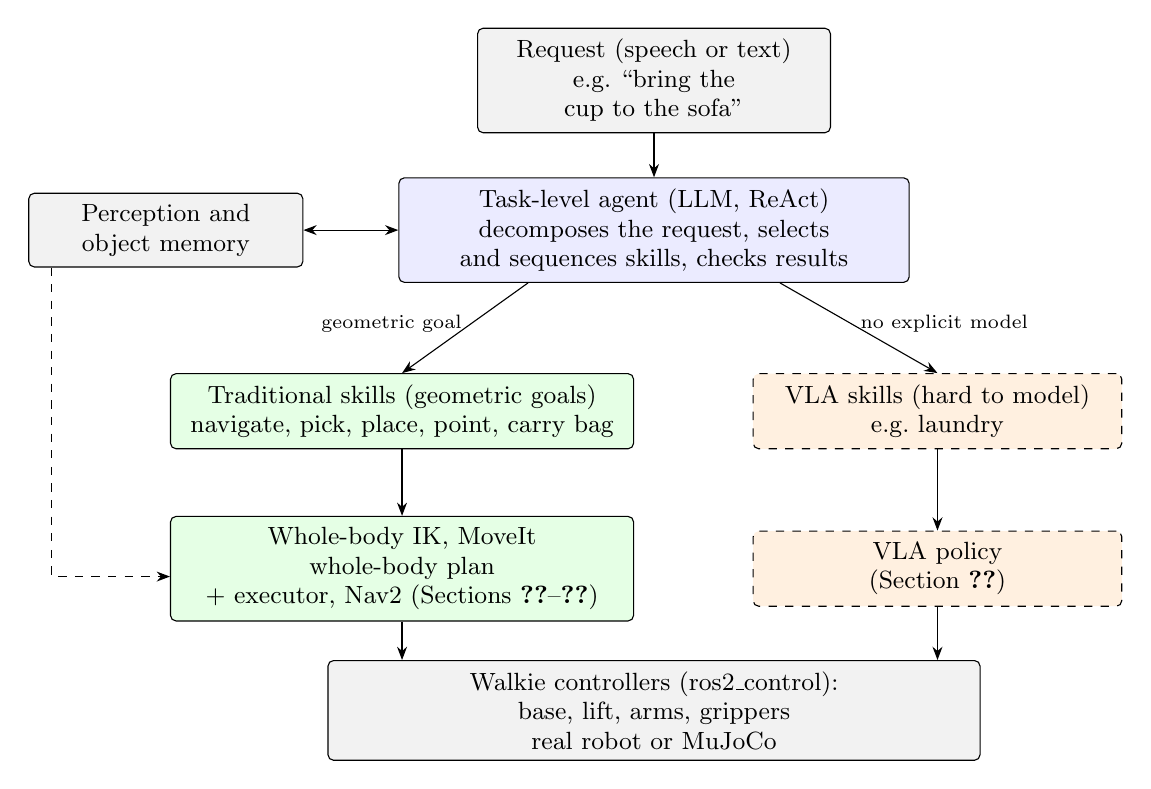
\begin{tikzpicture}[
        >=Stealth, font=\small,
        box/.style={draw, rounded corners=2pt, align=center, minimum height=9mm, text width=#1, inner sep=4pt,
                    execute at begin node=\setlength{\baselineskip}{1.15em}},
        box/.default=3.4cm]
        \node[box=4.2cm, fill=gray!10] (cmd) at (0,0) {Request (speech or text)\\e.g.\ ``bring the cup to the sofa''};
        \node[box=6.2cm, fill=blue!8] (agent) at (0,-1.9) {Task-level agent (LLM, ReAct)\\decomposes the request, selects and sequences skills, checks results};
        \node[box=3.2cm, fill=gray!10] (perc) at (-6.2,-1.9) {Perception and\\object memory};
        \node[box=5.6cm, fill=green!10] (trad) at (-3.2,-4.2) {Traditional skills (geometric goals)\\navigate, pick, place, point, carry bag};
        \node[box=4.4cm, fill=orange!12, dashed] (vla) at (3.6,-4.2) {VLA skills (hard to model)\\e.g.\ laundry};
        \node[box=5.6cm, fill=green!10] (wb) at (-3.2,-6.2) {Whole-body IK, MoveIt whole-body plan\\+ executor, Nav2 (Sections~\ref{sec:ik}--\ref{sec:planning})};
        \node[box=4.4cm, fill=orange!12, dashed] (pol) at (3.6,-6.2) {VLA policy\\(Section~\ref{sec:vla})};
        \node[box=8.0cm, fill=gray!10] (robot) at (0,-8.0) {Walkie controllers (ros2\_control): base, lift, arms, grippers\\real robot or MuJoCo};
        \draw[->] (cmd) -- (agent);
        \draw[<->] (perc) -- (agent);
        \draw[->] ([xshift=-1.6cm]agent.south) -- node[pos=0.45, left, font=\scriptsize]{geometric goal} (trad.north);
        \draw[->] ([xshift=1.6cm]agent.south) -- node[pos=0.45, right, font=\scriptsize]{no explicit model} (vla.north);
        \draw[->] (trad) -- (wb);
        \draw[->] (vla) -- (pol);
        \draw[->] (wb) -- (robot.north -| wb);
        \draw[->] (pol) -- (robot.north -| pol);
        \draw[->, dashed] (perc.south west) ++(0.3,0) |- ([yshift=-1mm]wb.west);
    \end{tikzpicture}
    \caption{\small{Hybrid architecture: the agent routes each skill to traditional coordinated base--arm
    control or to the VLA branch. Dashed boxes are in progress.}}
    \label{fig:arch}
\end{figure}

\subsection{Routing Between Traditional Control and VLA}

Most everyday requests can be reasoned out by the agent: it breaks them into steps such as going
somewhere, finding an object, grasping it and putting it down, and each step has a clear geometric
goal that traditional control can reach reliably, with collision checking and explicit failures the
agent can react to. Other tasks are hard to break down this way, because the objects deform, the
contacts are continuous, or the right next action depends on what the robot sees at every moment.
These are better handled by a VLA policy that has learned the task from demonstrations.

\begin{table}[H]
    \centering
    \small
    \renewcommand{\arraystretch}{1.2}
    \begin{tabular}{p{0.44\linewidth} p{0.44\linewidth}}
        \toprule
        Agent + traditional control & VLA \\
        \midrule
        Pick and place an object & Folding laundry \\
        Hand an object to a person & Wiping or cleaning a table \\
        Point at an object or person & Making a bed \\
        Carry a bag to a location & Loading a dishwasher \\
        Open a door or drawer of a known type & Tidying a cluttered room \\
        \midrule
        Clear geometric goals, rigid objects & Deformable objects, continuous contact \\
        \bottomrule
    \end{tabular}
    \caption{\small{Example tasks for each branch.}}
    \label{tab:routing}
\end{table}

\subsection{Task-Level Agent}

Task-level control was restructured from \texttt{walkie-agent-v2}, a LangChain/LangGraph multi-agent
application, into \texttt{walkie-agent-ros}, a ROS~2 node built on RAI's ReAct agent whose tools talk
to the robot through ROS topics, services and actions. It uses the same Pixi environment as the robot
software, accepts text or speech requests, and currently provides tools for speech, named-location
navigation (Nav2 goals with bounded waits and cancellation on timeout), bounded relative motion, pose
lookup and object-memory queries, with tests against a fake robot and a scripted language model. A
successor (\emph{Mahoraga}) that maintains an explicit task plan and discovers and composes typed
tools has been designed. In this architecture, the manipulation skills of Section~\ref{sec:skills} are
exposed to the agent as typed tools with explicit failure results (for example \emph{unreachable},
\emph{plan failed} or \emph{grasp not detected}), so the agent can re-plan at the task level when a
skill fails, while all motion-level decisions stay in the control stack.

% ============================================================
\section{Platform, Software and Simulation}
\label{sec:platform}

\subsection{The Walkie Platform}

The project extends Walkie, a mobile manipulator developed by the Engineer Innovator Club (EIC)
at Chulalongkorn University for RoboCup@Home, where it placed 6th of 25 teams in 2026. Walkie
has a four-wheel omnidirectional base, a vertical lift, and two 7-DOF OpenArm v10 arms with
parallel grippers, a head with a stereo camera and 3D lidar, and front and rear planar lidars
(Fig.~\ref{fig:walkie}). The project does not modify the hardware; it develops the
motion-planning layer.

\begin{figure}[H]
    \centering
    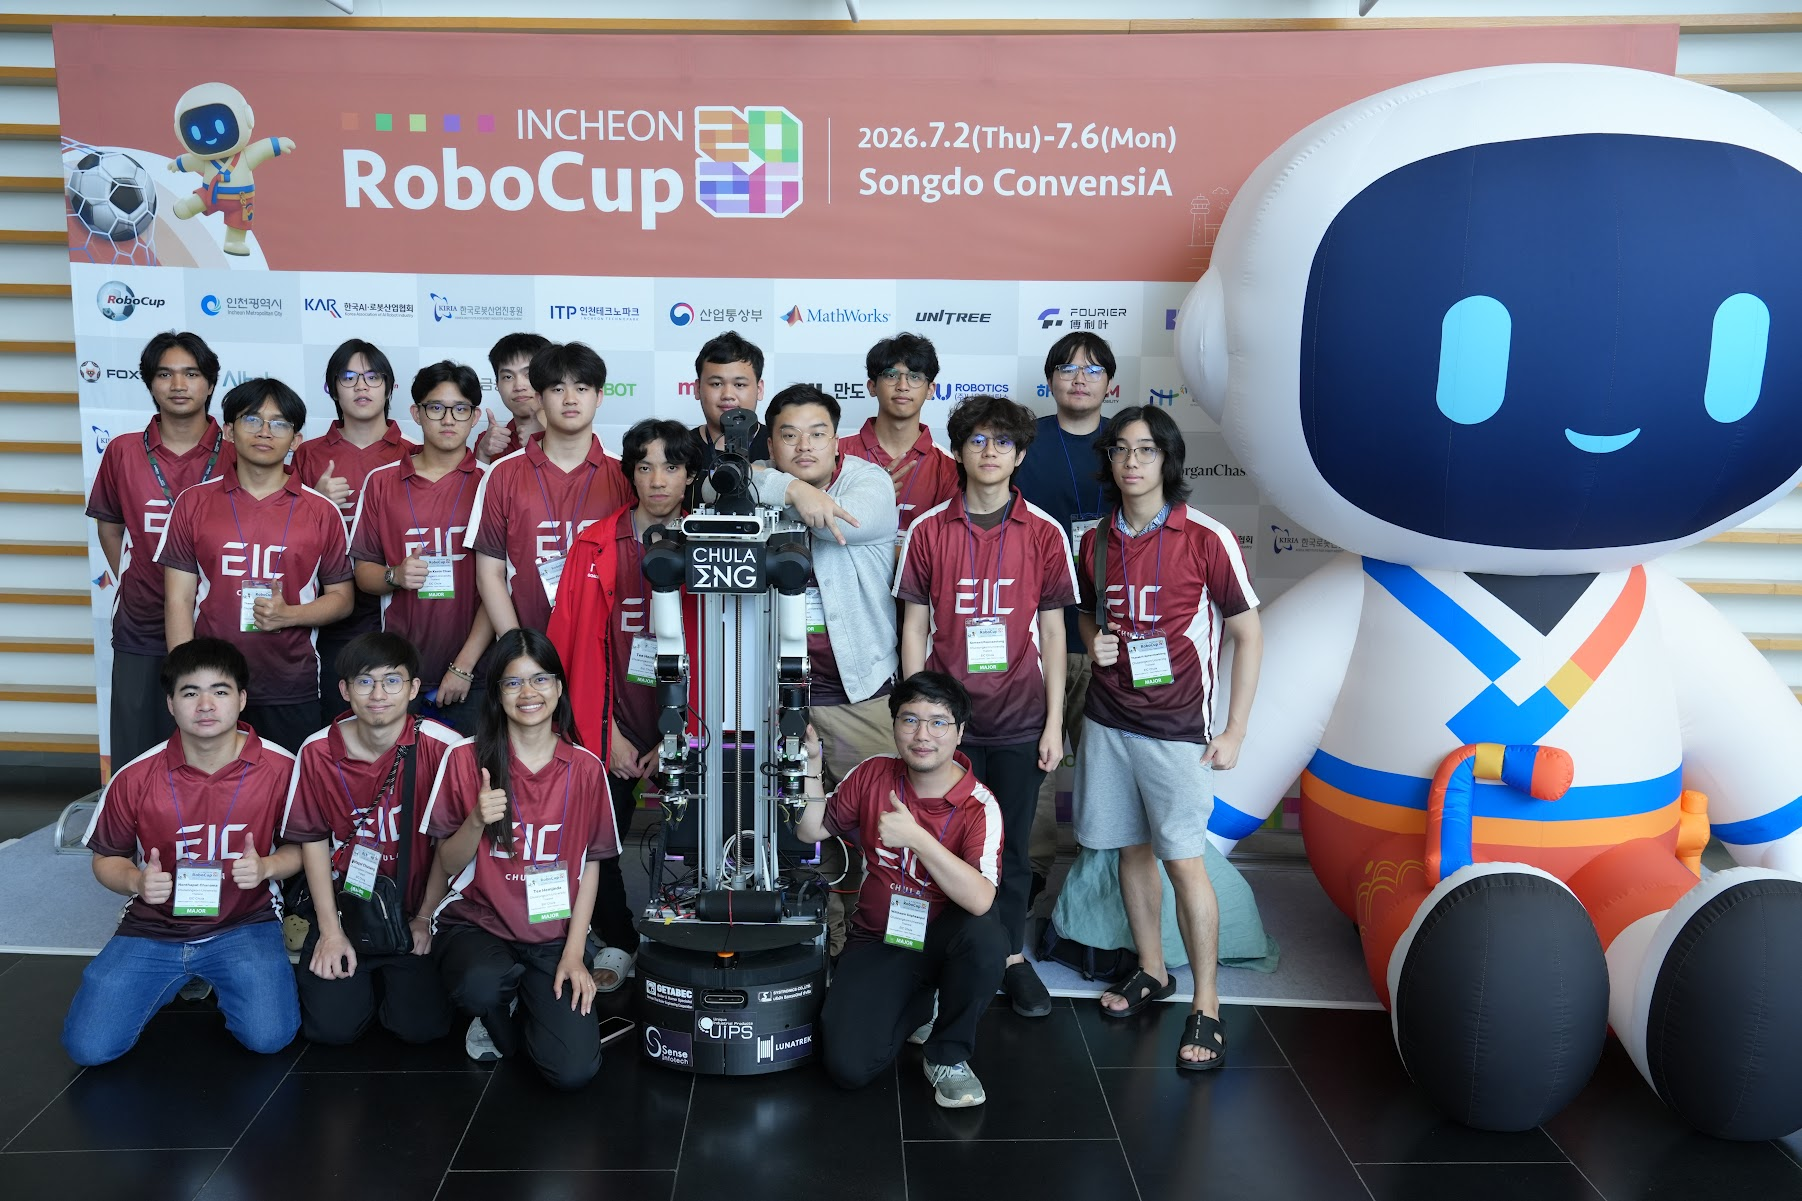
\includegraphics[width=0.62\linewidth]{DSC06194.jpg}
    \caption{\small{Walkie and the EIC RoboCup@Home team.}}
    \label{fig:walkie}
\end{figure}

For planning, the robot is described by the joint-state vector
\begin{equation}
    \mathbf{q} = [\,\mathbf{q}_B;\ \mathbf{q}_L;\ \mathbf{q}_R\,]
    = [\,x,\ y,\ \psi,\ z_l,\ q_{L_1},\dots,q_{L_7},\ q_{R_1},\dots,q_{R_7}\,]^{T}\in\mathbb{R}^{18}
    \label{eq:q18}
\end{equation}
where $(x, y, \psi)$ is the planar pose of the base in the map frame, $z_l$ the lift height, and
$\mathbf{q}_L$, $\mathbf{q}_R$ the left and right arm joints. The pose of a hand in the world frame is
the product of the base, lift, arm-mount and arm transforms,
\begin{equation}
    {}^{W}\mathbf{T}_{E}(\mathbf{q}) = {}^{W}\mathbf{T}_{B}(x,y,\psi)\;{}^{B}\mathbf{T}_{L}(z_l)\;
    {}^{L}\mathbf{T}_{A}\;{}^{A}\mathbf{T}_{E}(\mathbf{q}_{arm}).
    \label{eq:chain}
\end{equation}

\subsection{Development Path}

The work progressed through three simulation models, each closer to the real robot:
\begin{enumerate}
    \item \textbf{OpenArm with virtual base joints} (first progress report). An existing OpenArm
          MuJoCo model was extended with virtual prismatic and revolute joints for the base
          ($x$, $y$, lift, yaw) to test the unified kinematic model (Fig.~\ref{fig:early_models}a).
    \item \textbf{Walker model with DH kinematics} (second progress report). Forward kinematics
          was written as a Denavit--Hartenberg chain of the base and arm, and the IK solver was
          developed and benchmarked on this model (Section~\ref{sec:ik}).
    \item \textbf{Full Walkie simulation} (this report). The solver was moved onto the MuJoCo model
          generated from Walkie's own robot description, running under ROS~2 with Nav2 and MoveIt
          (Section~\ref{sec:walkie}).
\end{enumerate}

\begin{figure}[H]
    \centering
    \begin{subfigure}[t]{0.48\textwidth}
        \centering
        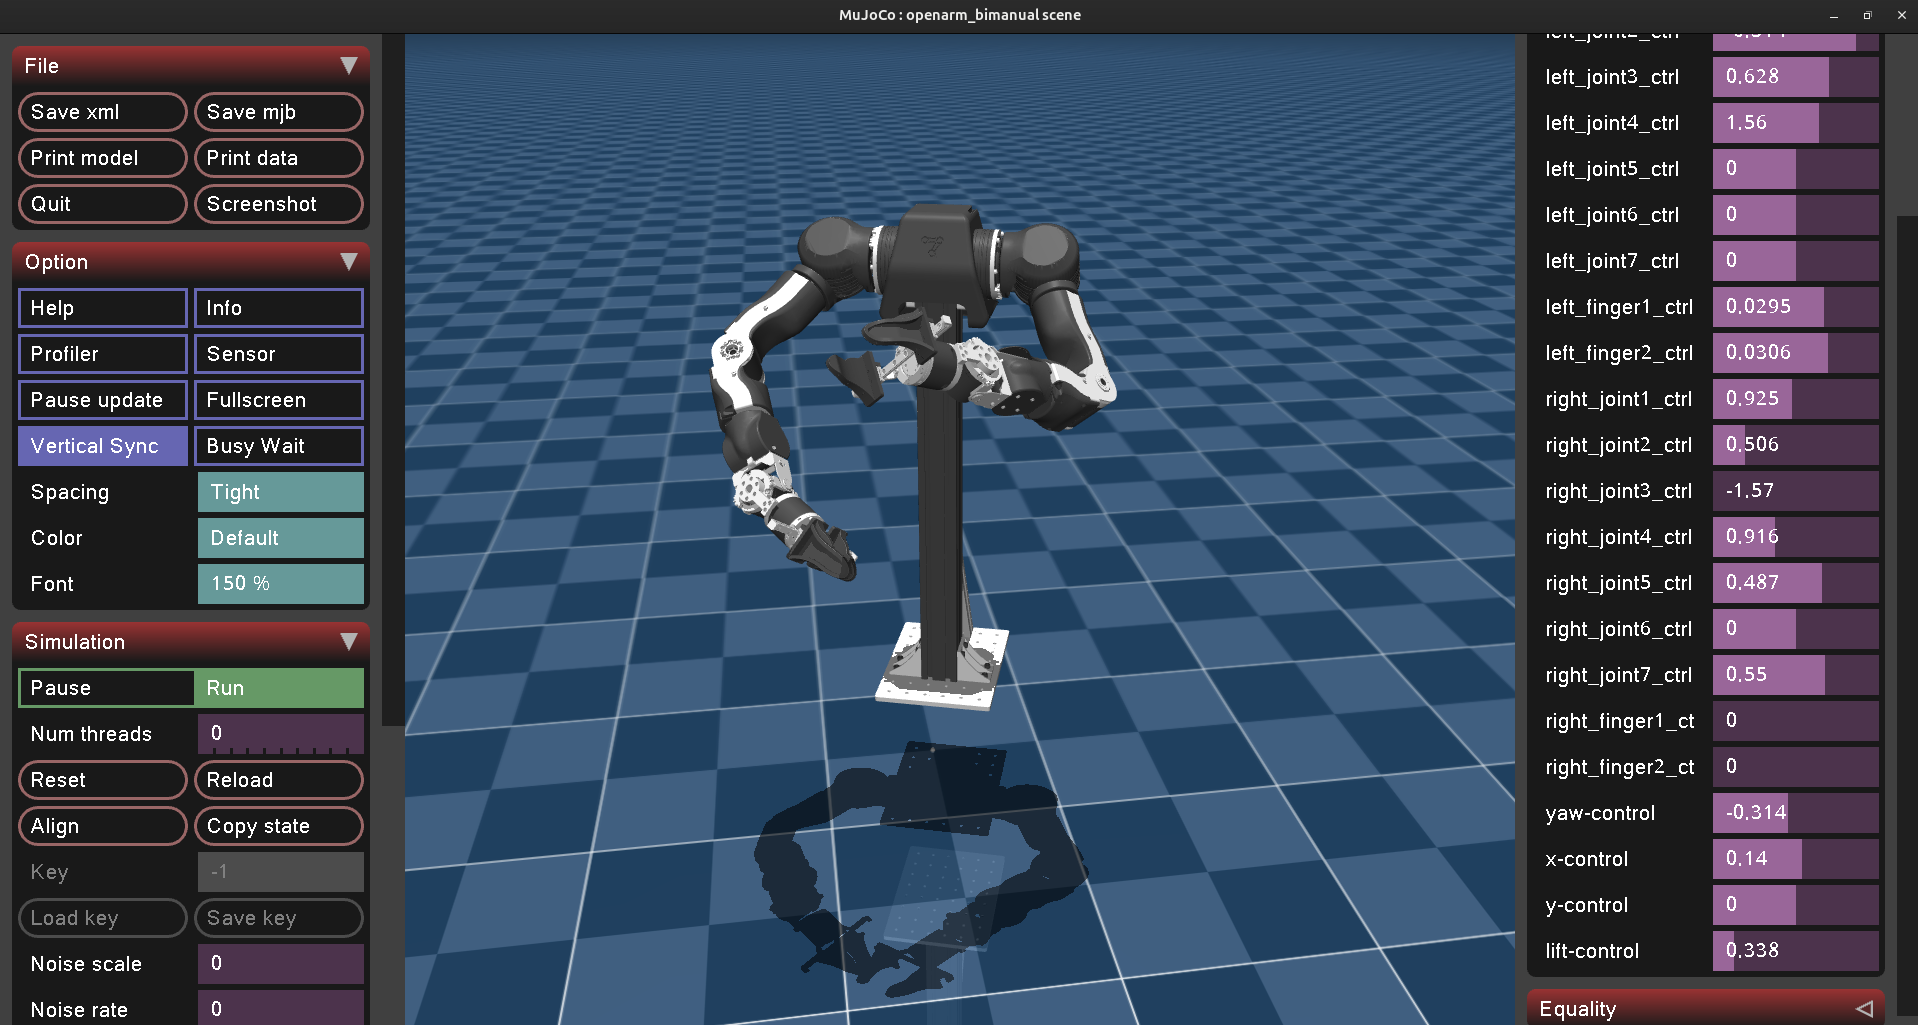
\includegraphics[height=4.6cm]{Mujoco_walker.png}
        \caption{OpenArm with virtual base joints}
    \end{subfigure}\hfill
    \begin{subfigure}[t]{0.48\textwidth}
        \centering
        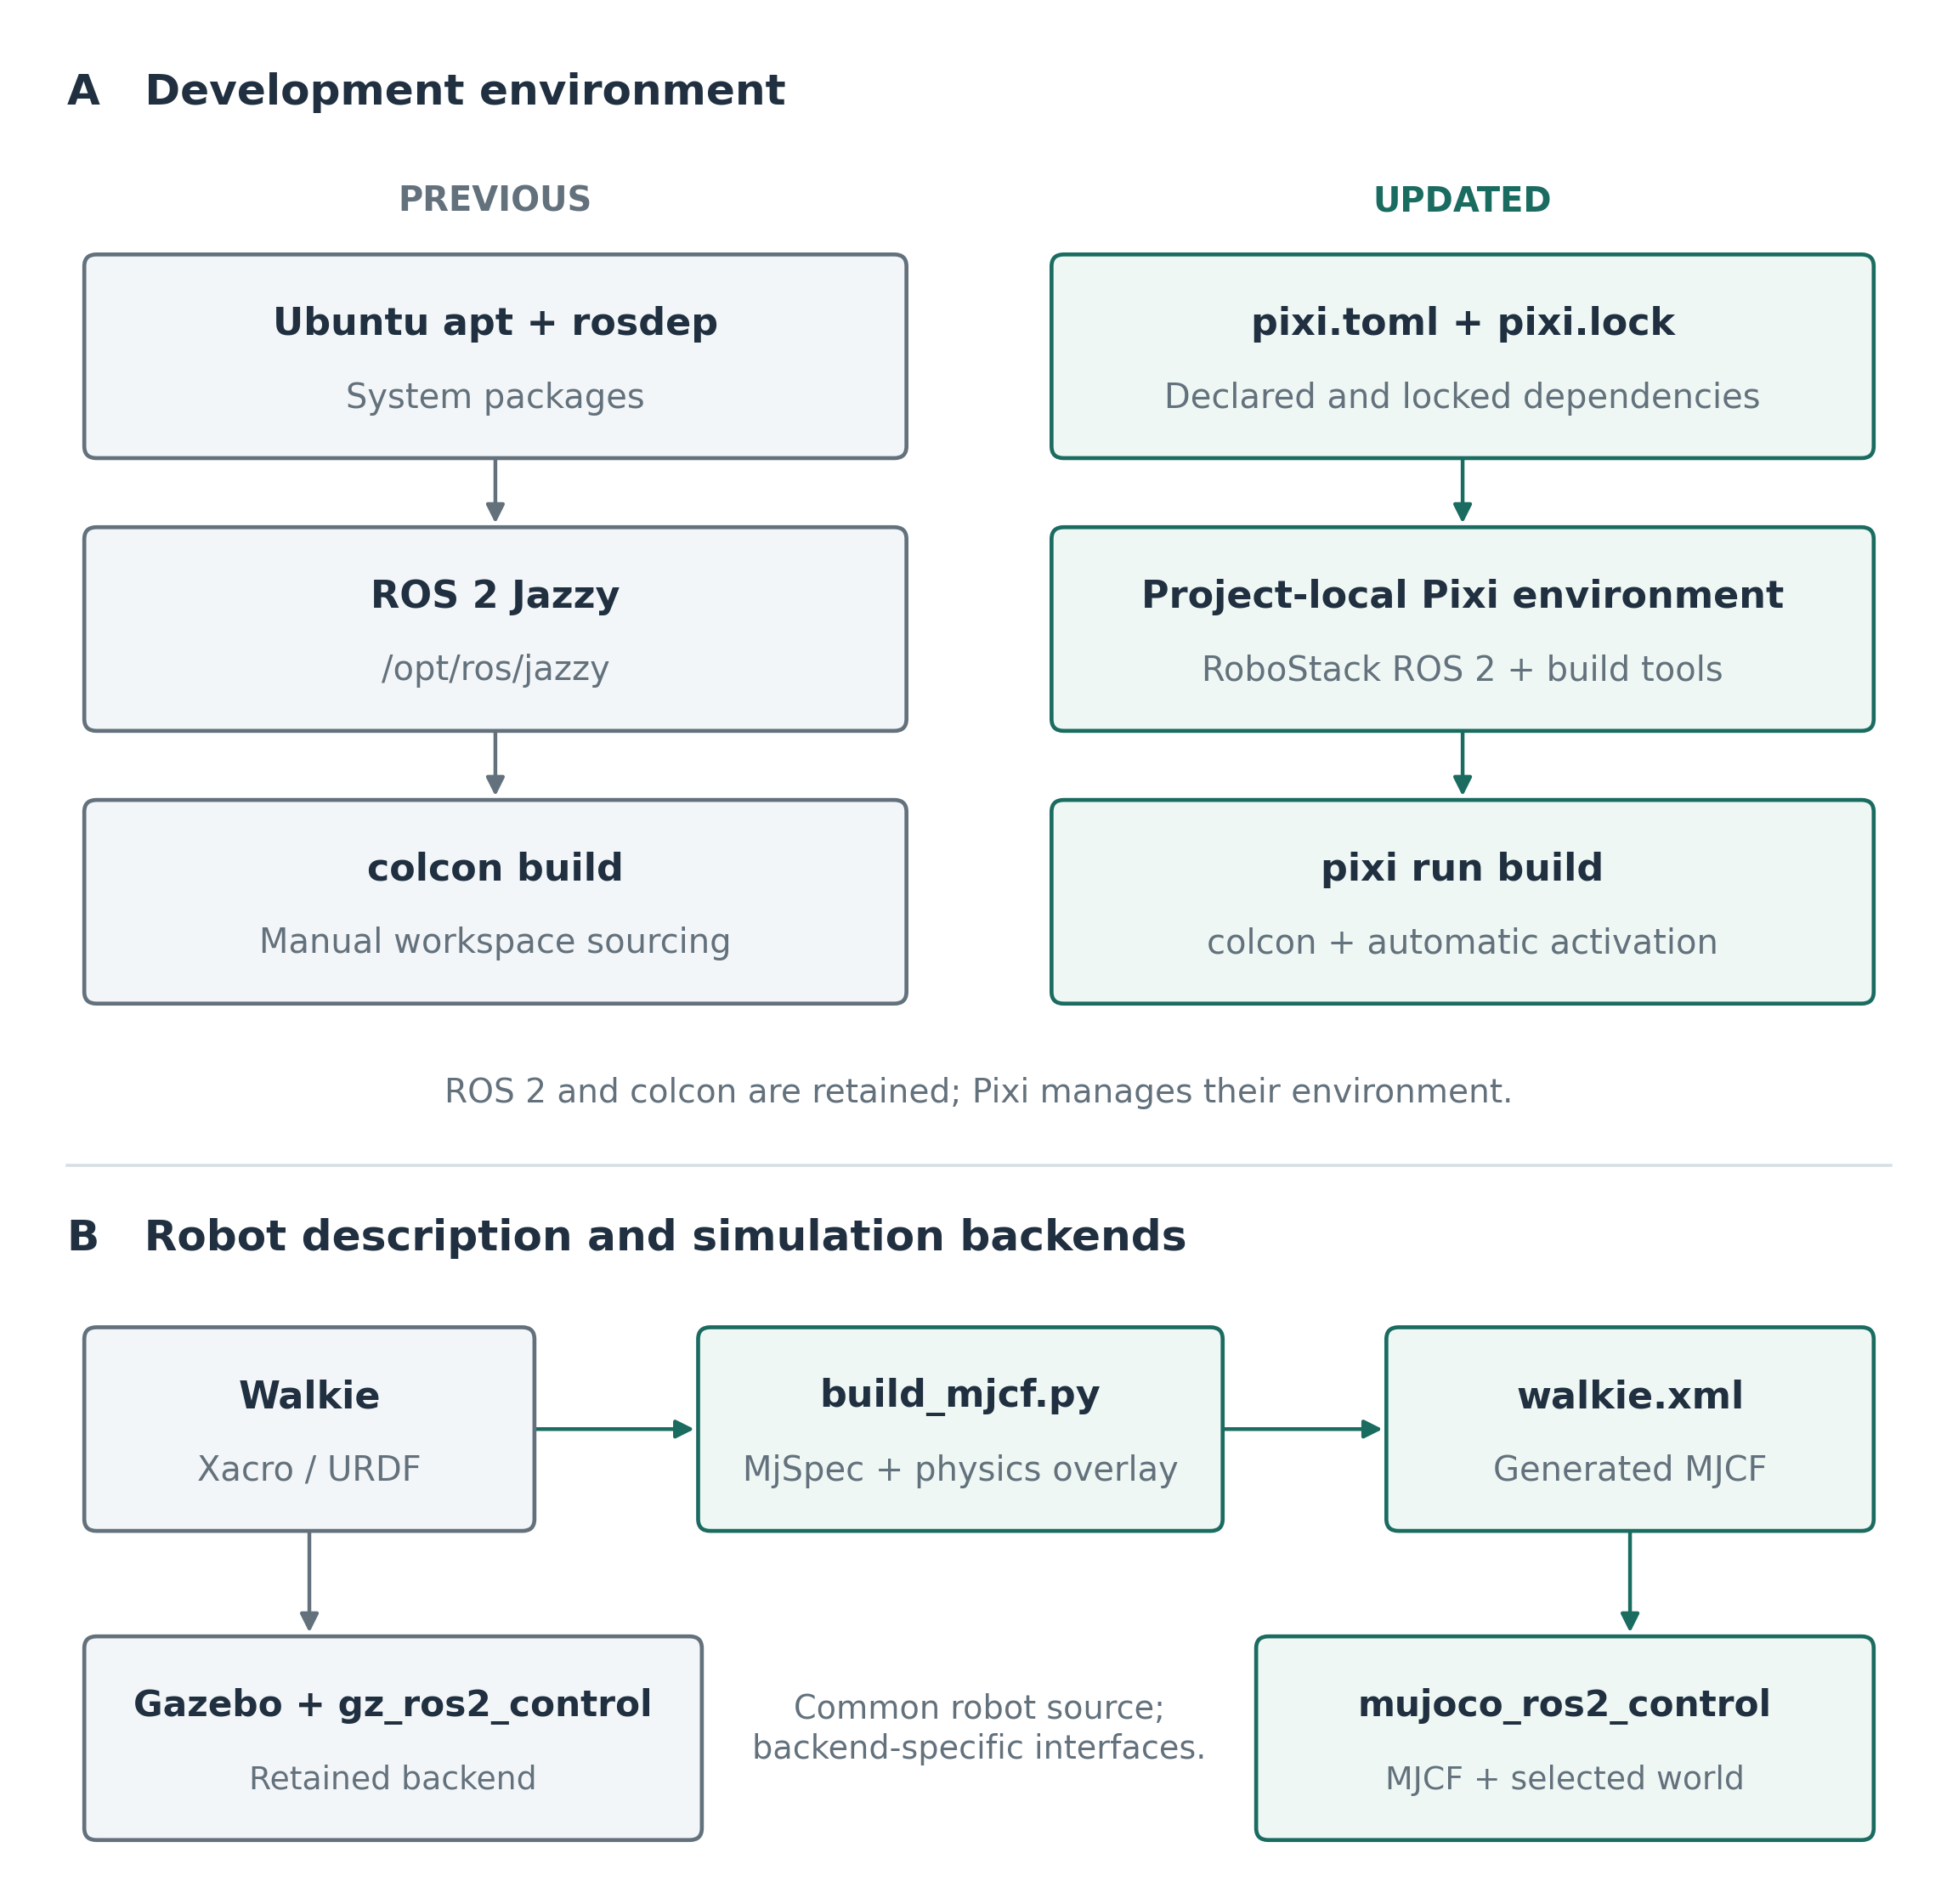
\includegraphics[height=4.6cm]{migration_gazebo_mujoco_comparison.png}
        \caption{Walkie in Gazebo and in MuJoCo}
    \end{subfigure}
    \caption{\small{Simulation models used during the project.}}
    \label{fig:early_models}
\end{figure}

\subsection{Software Environment}

The robot software lives in the \texttt{walkie-ros} repository. It was moved from a
system-wide ROS~2 Jazzy installation to a project-local Pixi environment built from the
RoboStack and conda-forge channels, with every dependency pinned in a lockfile. ROS~2 remains the
middleware (with Zenoh as the RMW layer) and \texttt{colcon} the build tool; Pixi provides
reproducible installation, build and test commands. The migration required pinning the compiler
and CMake versions, fixing the navigation stack's OpenVDB and Boost dependencies, and aligning the
ROS packages with a RoboStack build set that provides the MuJoCo control plugin.

\subsection{MuJoCo Simulation of Walkie}

A MuJoCo model is generated from the same Xacro/URDF description as the real robot, so the
simulated and real kinematics cannot drift apart. The generator adds a floating base,
actuators, collision classes, sensors and a home keyframe. The omnidirectional wheels are thin
capsules on an analytic floor with direction-dependent friction, so that the wheel velocity
controllers drive the floating base through contact forces rather than by setting its pose; this
work also corrected the wheel distance in the controller from 0.252\,m to 0.185\,m. The model is
connected to ROS~2 through \texttt{mujoco\_ros2\_control} with the same controllers as the real
robot, and publishes the IMU, cameras, both planar lidars (merged for Nav2) and the head 3D lidar.
Named worlds can be loaded with their own occupancy map and AMCL localisation; the first is a
reconstruction of the Chulapat~14 living room and kitchen (Fig.~\ref{fig:world}). Automated tests
check the description, the controller interfaces, the generated model, the URDF--SRDF contract and
every installed world.

\begin{figure}[H]
    \centering
    \begin{subfigure}[t]{0.55\textwidth}
        \centering
        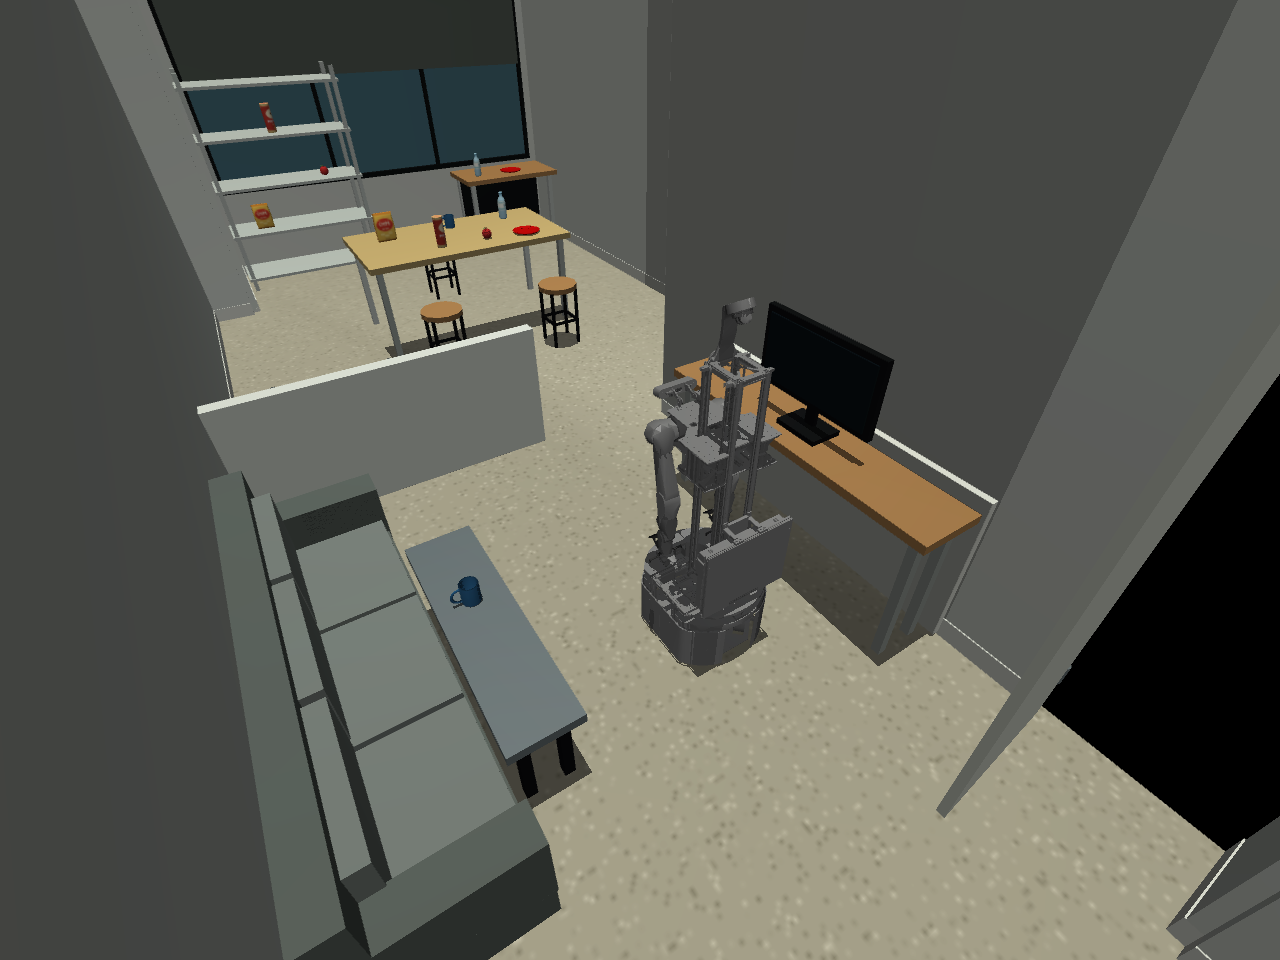
\includegraphics[height=5cm]{migration_walkie_mujoco_room.png}
        \caption{Walkie in the reconstructed room}
    \end{subfigure}\hfill
    \begin{subfigure}[t]{0.42\textwidth}
        \centering
        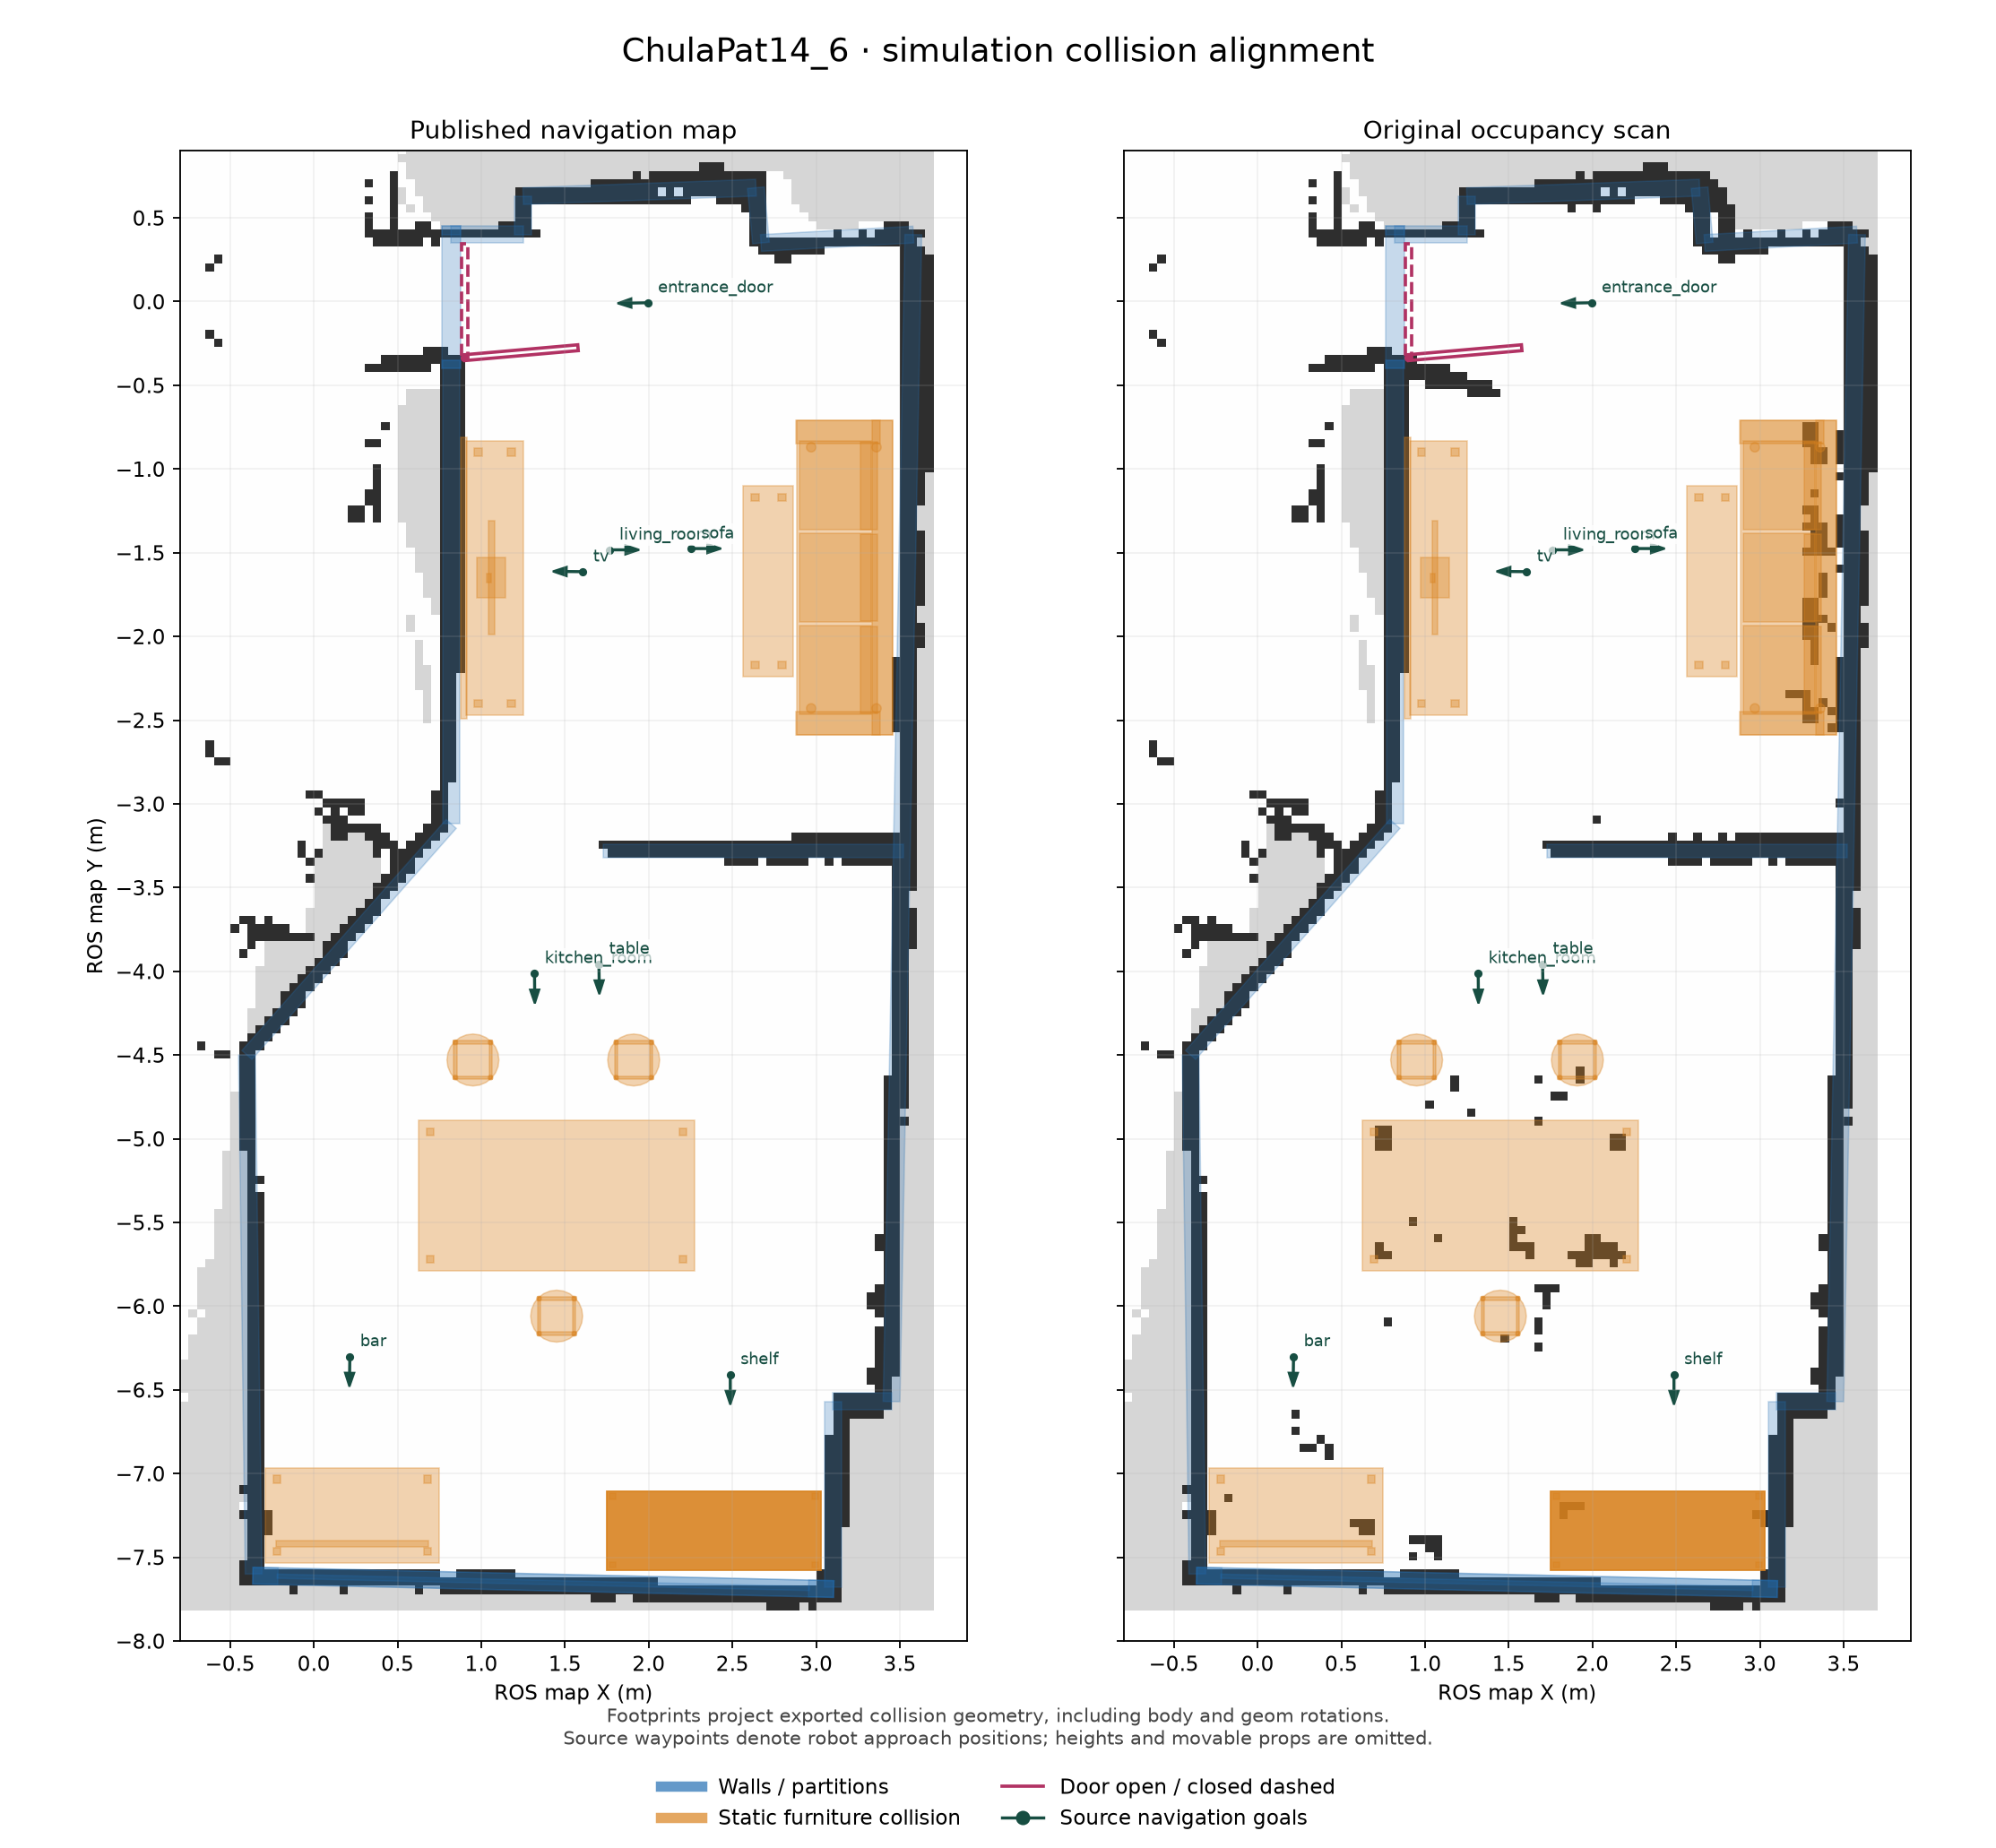
\includegraphics[height=5cm]{chula_map_alignment.png}
        \caption{World geometry over its Nav2 map}
    \end{subfigure}
    \caption{\small{The Chulapat~14 named world.}}
    \label{fig:world}
\end{figure}

% ============================================================
\section{Whole-Body Inverse Kinematics}
\label{sec:ik}

This section summarises how the IK solver was developed on the Walker model. The derivations
were introduced in the second progress report; here they are consolidated and the results of the
final benchmark are added (Section~\ref{sec:ik_bench}).

\subsection{Forward and Differential Kinematics}

On the Walker model the forward kinematics of the base and left arm was written as a standard
Denavit--Hartenberg chain of 24 frames (the base coordinates enter as joint variables), with
\begin{equation}
    {}^{i-1}\mathbf{T}_{i} =
    \begin{bmatrix}
        \cos\theta_i & -\sin\theta_i\cos\alpha_i & \sin\theta_i\sin\alpha_i & a_i\cos\theta_i\\
        \sin\theta_i & \cos\theta_i\cos\alpha_i & -\cos\theta_i\sin\alpha_i & a_i\sin\theta_i\\
        0 & \sin\alpha_i & \cos\alpha_i & d_i\\
        0 & 0 & 0 & 1
    \end{bmatrix},
    \qquad
    {}^{0}\mathbf{T}_{n} = {}^{0}\mathbf{T}_{1}\,{}^{1}\mathbf{T}_{2}\cdots{}^{n-1}\mathbf{T}_{n}.
\end{equation}
The hand position $\mathbf{p}(\mathbf{q})$ and orientation $\mathbf{R}(\mathbf{q})$ are read from
${}^{0}\mathbf{T}_{n}$, and the geometric Jacobian relates joint and hand velocities,
\begin{equation}
    \begin{bmatrix}\dot{\mathbf{p}}\\ \boldsymbol{\omega}\end{bmatrix}
    = \begin{bmatrix}\mathbf{J}_v(\mathbf{q})\\ \mathbf{J}_\omega(\mathbf{q})\end{bmatrix}\dot{\mathbf{q}}.
\end{equation}
Each IK iteration replaces the velocity by the error to the target,
$\mathbf{e}_p = \mathbf{p}_{\mathrm{target}}-\mathbf{p}(\mathbf{q}_k)$, and the orientation error
$\mathbf{e}_\omega$ is the rotation vector of $\mathbf{R}_{\mathrm{target}}\mathbf{R}(\mathbf{q}_k)^{T}$.
The update $\mathbf{q}_{k+1}=\mathbf{q}_k+\Delta\mathbf{q}$ is repeated until the error is below
tolerance.

\subsection{From Pseudoinverse to Damped Least Squares}

The pseudoinverse $\Delta\mathbf{q}=\mathbf{J}^{\dagger}\mathbf{e}$, with
$\mathbf{J}^{\dagger}=\mathbf{J}^{T}(\mathbf{J}\mathbf{J}^{T})^{-1}$, is the minimum-norm least-squares
step~\cite{buss2009}. Near a singularity $\mathbf{J}\mathbf{J}^{T}$ is nearly singular and the step
becomes very large. Damped least squares regularises it,
\begin{equation}
    \min_{\Delta\mathbf{q}}\ \|\mathbf{e}-\mathbf{J}\Delta\mathbf{q}\|^2 + \lambda^2\|\Delta\mathbf{q}\|^2
    \quad\Rightarrow\quad
    \Delta\mathbf{q} = \mathbf{J}^{T}\left(\mathbf{J}\mathbf{J}^{T}+\lambda^2\mathbf{I}\right)^{-1}\mathbf{e},
\end{equation}
which bounds the step at the cost of slower convergence (Fig.~\ref{fig:singularity}).

\begin{figure}[H]
    \centering
    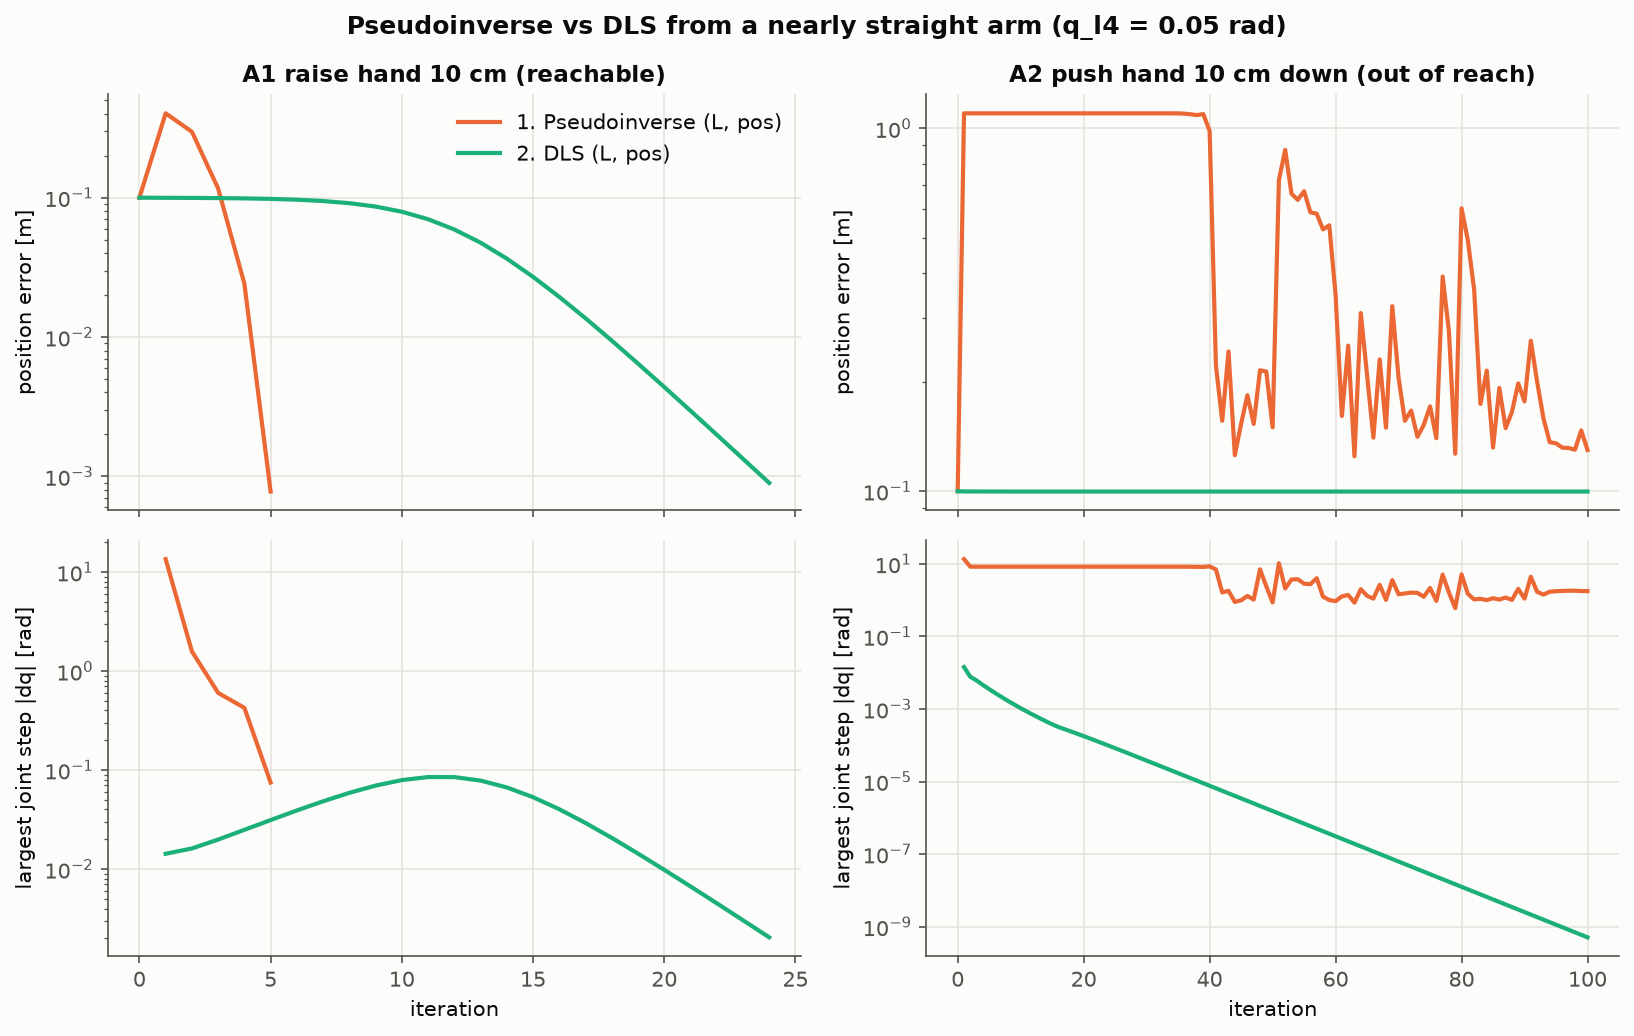
\includegraphics[width=0.85\linewidth]{A_singularity.png}
    \caption{\small{Pseudoinverse versus DLS from a nearly straight arm (elbow at 0.05\,rad).
    Left: a reachable target 10\,cm above the hand. The pseudoinverse converges in 5 iterations but
    its first step is over 10\,rad. Right: a target out of reach. The pseudoinverse oscillates with
    steps of several radians, while DLS stays at the closest reachable point with vanishing steps.
    Video: \vidlink{https://youtu.be/MEW62I4-9JQ}{comparison}.}}
    \label{fig:singularity}
\end{figure}

\subsection{Per-Joint and Joint-Limit Damping}

A single $\lambda$ treats a metre of base motion and a radian of arm motion alike. Following the
dynamic weighting of Schinstock et al.~\cite{schinstock1994}, each joint gets its own damping,
$\boldsymbol{\Lambda}=\operatorname{diag}(\lambda_1^2,\dots,\lambda_n^2)$, and is additionally
weighted by $w_i\ge 1$ when it moves towards a limit:
\begin{equation}
    \left(\mathbf{J}^{T}\mathbf{J}+\boldsymbol{\Lambda}\mathbf{W}\right)\Delta\mathbf{q}=\mathbf{J}^{T}\mathbf{e},
    \qquad
    \mathbf{W}=\operatorname{diag}(w_i).
    \label{eq:weighted_dls}
\end{equation}
With $d_i$ the normalised distance of joint $i$ to the limit it is heading towards, $m$ the margin
(as a fraction of the joint range) and $g$ a gain,
\begin{equation}
    p_i=\operatorname{clip}\!\left(\frac{m-d_i}{m},0,1\right),
    \qquad
    w_i=1+g\,\frac{p_i^2}{1-p_i+\varepsilon}.
    \label{eq:limit_weight}
\end{equation}
Outside the margin, or when moving away from the limit, $w_i=1$; at the limit the joint is
effectively frozen. Because $w_i$ depends on the sign of $\Delta q_i$, the system is solved
$n_r=2$ times, each time recomputing $\mathbf{W}$ from the previous step, and the result is clipped
to the limits. Base damping ($\lambda=0.6$) is set higher than arm damping ($\lambda=0.2$) so that
the arms do most of the work and the base moves only when the arms need it.

\subsection{Rest Posture as a Soft Weight}

With 11 joints and a 3D position task, the solution is not unique and the arm can drift into
awkward postures. The first remedy added a cost
$(\Delta\mathbf{q}+\boldsymbol{\delta})^{T}\mathbf{R}(\Delta\mathbf{q}+\boldsymbol{\delta})$ on the
offset $\boldsymbol{\delta}=\mathbf{q}-\mathbf{q}^{\mathrm{rest}}$, giving
\begin{equation}
    \left(\mathbf{J}^{T}\mathbf{J}+\boldsymbol{\Lambda}\mathbf{W}+\mathbf{R}\right)\Delta\mathbf{q}
    = \mathbf{J}^{T}\mathbf{e}-\mathbf{R}\boldsymbol{\delta}.
    \label{eq:rest_normal}
\end{equation}
At convergence ($\Delta\mathbf{q}=\mathbf{0}$) this requires $\mathbf{J}^{T}\mathbf{e}=\mathbf{R}\boldsymbol{\delta}$:
the damping does not move the equilibrium, but the rest pull does, leaving a residual error that
grows with $\mathbf{R}$. For a single arm with a small weight this works well (Fig.~\ref{fig:rest_single}),
but it fails with two arms (next subsection).

\begin{figure}[H]
    \centering
    \begin{subfigure}[t]{0.48\textwidth}
        \centering
        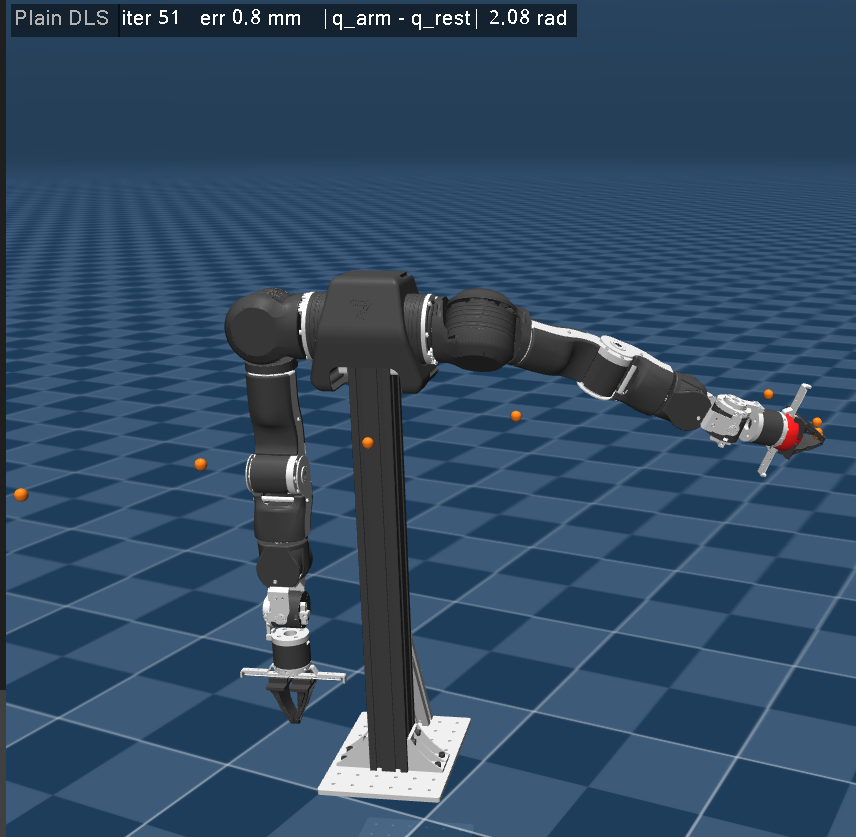
\includegraphics[height=5.5cm]{plain_dls.png}
        \caption{Per-joint DLS only}
    \end{subfigure}\hfill
    \begin{subfigure}[t]{0.48\textwidth}
        \centering
        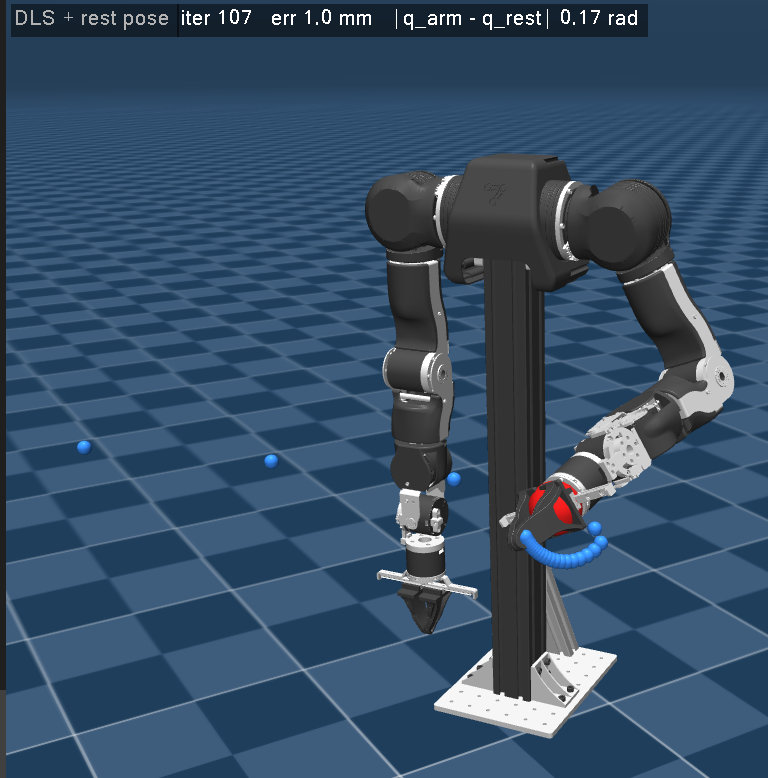
\includegraphics[height=5.5cm]{rest_dls.png}
        \caption{With the rest pull}
    \end{subfigure}
    \caption{\small{Single arm, same target: the rest pull keeps the arm near its rest posture
    and the base takes up more of the motion (\vidlink{https://youtu.be/wrWfXNqLJrA}{video}).}}
    \label{fig:rest_single}
\end{figure}

\subsection{Two Arms Sharing the Base: the Stacked Solve}

With both arms, the two hand Jacobians share the base columns,
$\mathbf{J}_L=[\mathbf{B}_L\ \mathbf{A}_L\ \mathbf{0}]$ and $\mathbf{J}_R=[\mathbf{B}_R\ \mathbf{0}\ \mathbf{A}_R]$.
Solving each arm separately and averaging the two base steps fails: each arm compensates for a base
motion that is not the one applied, and when the two targets need opposite base motions the two
steps cancel. In the second progress report this stalled in 39 of 40 random target pairs. Writing
both tasks in one system instead~\cite{bussKim2004},
\begin{equation}
    \underbrace{\begin{bmatrix}\mathbf{e}_L\\ \mathbf{e}_R\end{bmatrix}}_{\mathbf{e}}
    \approx
    \underbrace{\begin{bmatrix}\mathbf{B}_L & \mathbf{A}_L & \mathbf{0}\\ \mathbf{B}_R & \mathbf{0} & \mathbf{A}_R\end{bmatrix}}_{\mathbf{J}}
    \Delta\mathbf{q},
    \qquad
    \mathbf{J}^{\#}=\left(\mathbf{J}^{T}\mathbf{J}+\boldsymbol{\Lambda}\mathbf{W}\right)^{-1}\mathbf{J}^{T},
    \label{eq:stacked}
\end{equation}
yields one step that reduces both errors together. With orientation, each hand contributes six
rows, and row and column selection matrices $\mathbf{S}_t$, $\mathbf{S}_q$ switch hands, orientation
and the base and lift on or off within the same solve,
$\Delta\mathbf{q}=\mathbf{S}_q(\mathbf{J}_{\mathrm{sel}}^{T}\mathbf{J}_{\mathrm{sel}}+\boldsymbol{\Lambda}_{\mathrm{sel}}\mathbf{W}_{\mathrm{sel}})^{-1}\mathbf{J}_{\mathrm{sel}}^{T}\mathbf{e}_{\mathrm{sel}}$
with $\mathbf{J}_{\mathrm{sel}}=\mathbf{S}_t\mathbf{J}\mathbf{S}_q$. Table~\ref{tab:modes} lists the
redundancy left in each mode.

\begin{table}[H]
    \centering
    \small
    \begin{tabular}{lccc}
        \toprule
        Mode & Rows & Joints & Spare DOF \\
        \midrule
        Both hands, position, base and lift on & 6 & 18 & 12 \\
        Both hands, pose, base and lift on & 12 & 18 & 6 \\
        Both hands, pose, base and lift off & 12 & 14 & 2 \\
        One hand, pose, base and lift on & 6 & 11 & 5 \\
        One hand, pose, base and lift off & 6 & 7 & 1 \\
        \bottomrule
    \end{tabular}
    \caption{\small{Task rows, enabled joints and spare degrees of freedom (assuming full rank).}}
    \label{tab:modes}
\end{table}

\subsection{Posture as a Null-Space Task}

The soft rest weight cannot be tuned for two arms: a weight small enough to reach both targets
($\le10^{-4}$) leaves the posture unchanged, and a larger one stalls with a residual error that
grows with the weight (16.7\,mm at $4\times10^{-3}$). The redundancy in Table~\ref{tab:modes} allows
a different treatment: following the task-priority framework of Nakamura et
al.~\cite{nakamura1987}, the posture acts only on joint motions that do not move the hands,
\begin{equation}
    \Delta\mathbf{q}
    = \mathbf{J}^{\#}\mathbf{e}
    + \left(\mathbf{I}-\mathbf{J}^{\#}\mathbf{J}\right)\mathbf{K}\left(\mathbf{q}^{\mathrm{des}}-\mathbf{q}\right),
    \label{eq:nullspace}
\end{equation}
where $\mathbf{K}$ is a diagonal gain. In the implementation $\mathbf{J}^{\#}\mathbf{J}$ is replaced
by a soft projector built from the singular value decomposition of $\mathbf{J}$ with slightly damped
singular values, so near-singular directions are not treated as free; the projector choice
distorts the secondary motion somewhat~\cite{lenarcic1998}. Because the posture term no longer
competes with the task, the equilibrium is at zero task error.

\begin{figure}[H]
    \centering
    \begin{subfigure}[t]{0.48\textwidth}
        \centering
        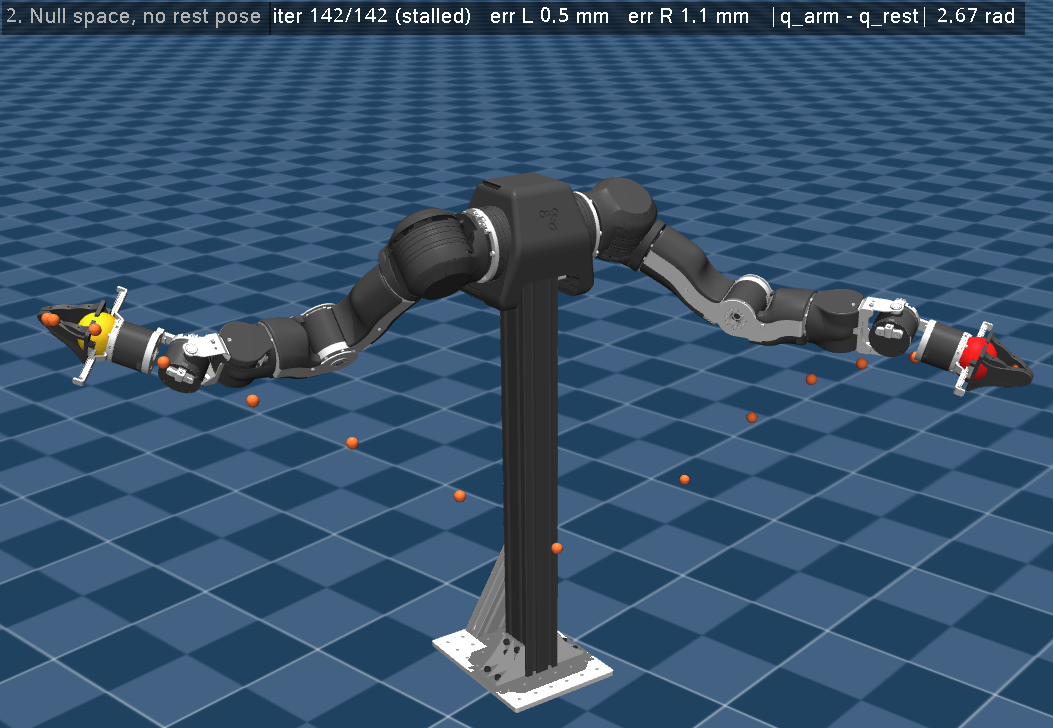
\includegraphics[height=4.6cm]{nullplain.png}
        \caption{No posture term}
    \end{subfigure}\hfill
    \begin{subfigure}[t]{0.48\textwidth}
        \centering
        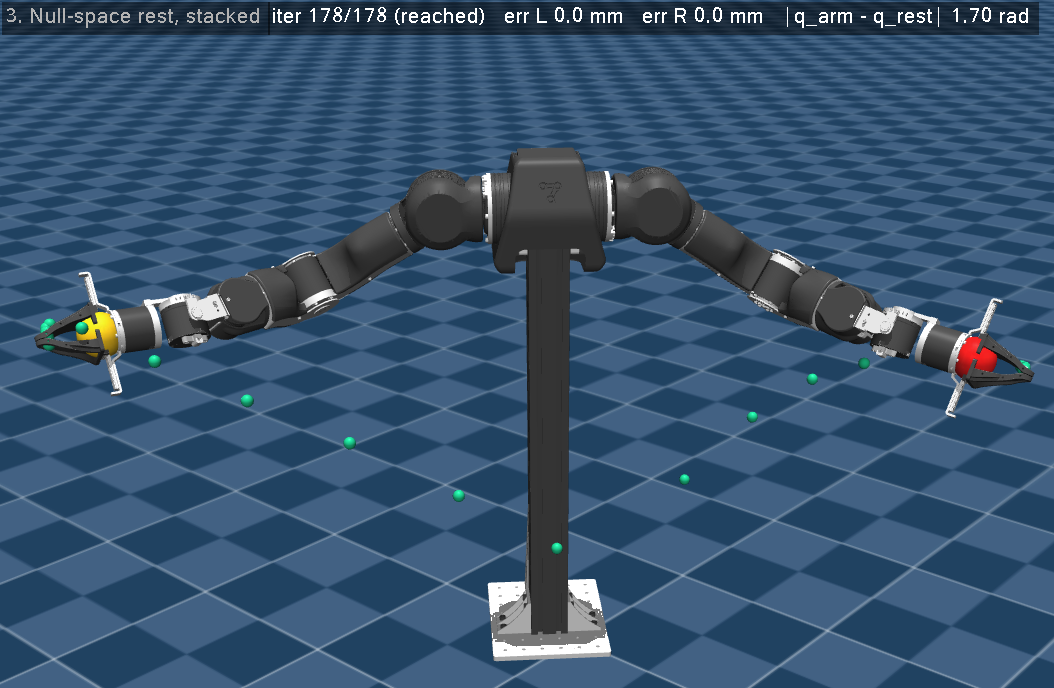
\includegraphics[height=4.6cm]{nullrest.png}
        \caption{Null-space rest posture}
    \end{subfigure}
    \caption{\small{Same two-hand target: both reach it, but the posture term keeps the arms near
    rest using only motions that do not move the hands (\vidlink{https://youtu.be/3rgqf_vf3_w}{video}).}}
    \label{fig:nullspace}
\end{figure}

\subsection{Offline Benchmark of the Solver Versions}
\label{sec:ik_bench}

The five solver stages were compared on the Walker model with a common benchmark
(\texttt{benchmark/run\_benchmark.py}). Each method is iterated from the same start until the
position error is below 1\,mm (and the orientation error below 0.5$^\circ$ for pose targets), or for at
most 300 iterations, without a step cap, so the numbers describe the solver rather than the
controller. Experiment B (Fig.~\ref{fig:bench_b}) runs stages 3--5 on one bimanual target that needs
the base and lift; experiment C (Fig.~\ref{fig:bench_c}, Table~\ref{tab:bench_c}) uses 200 random
reachable targets.

\begin{figure}[H]
    \centering
    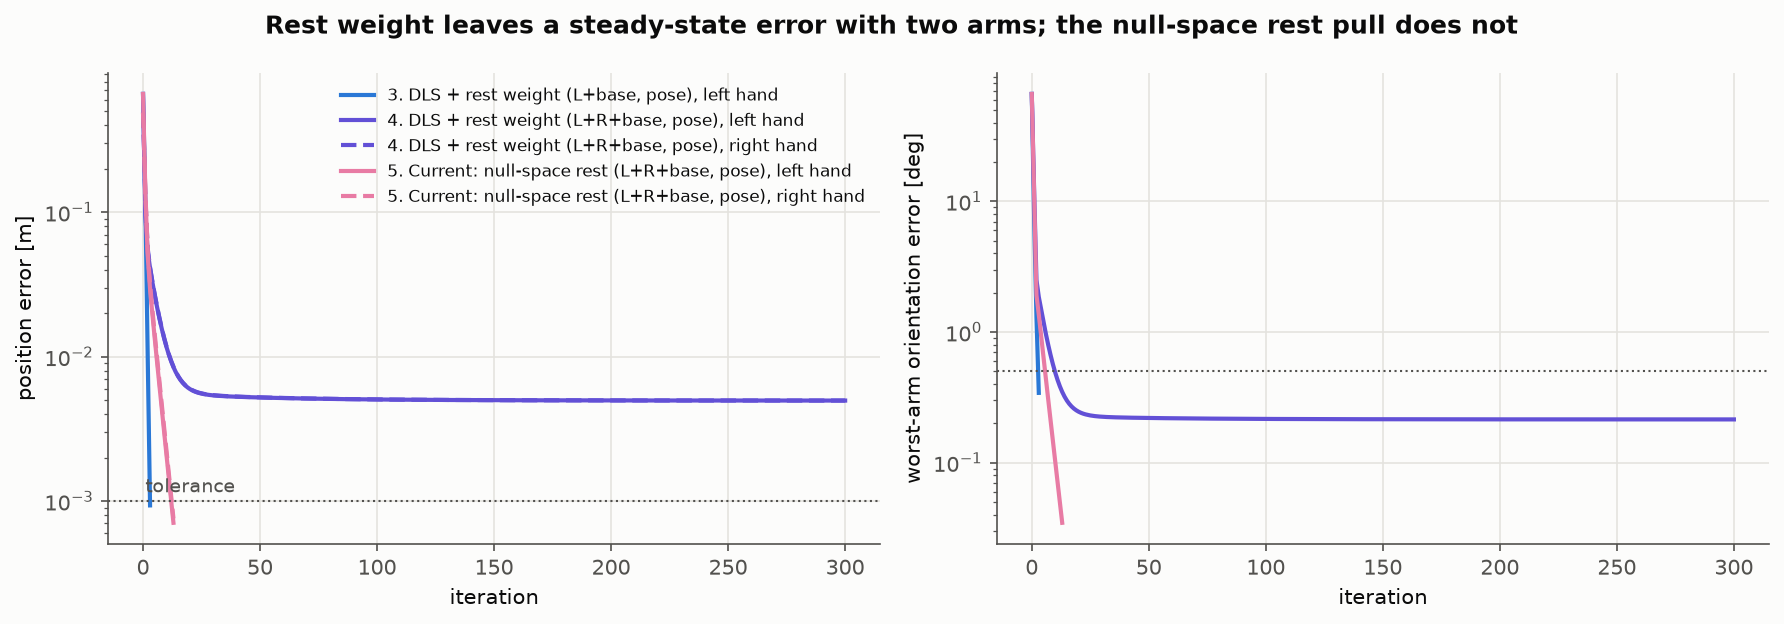
\includegraphics[width=0.95\linewidth]{B_rest_weight.png}
    \caption{\small{Experiment B. With two arms, the soft rest weight (stage 4) settles about 5\,mm and
    0.2$^\circ$ from the target and stays there; the null-space rest pull (stage 5) reaches tolerance in
    about 13 iterations.}}
    \label{fig:bench_b}
\end{figure}

\begin{figure}[H]
    \centering
    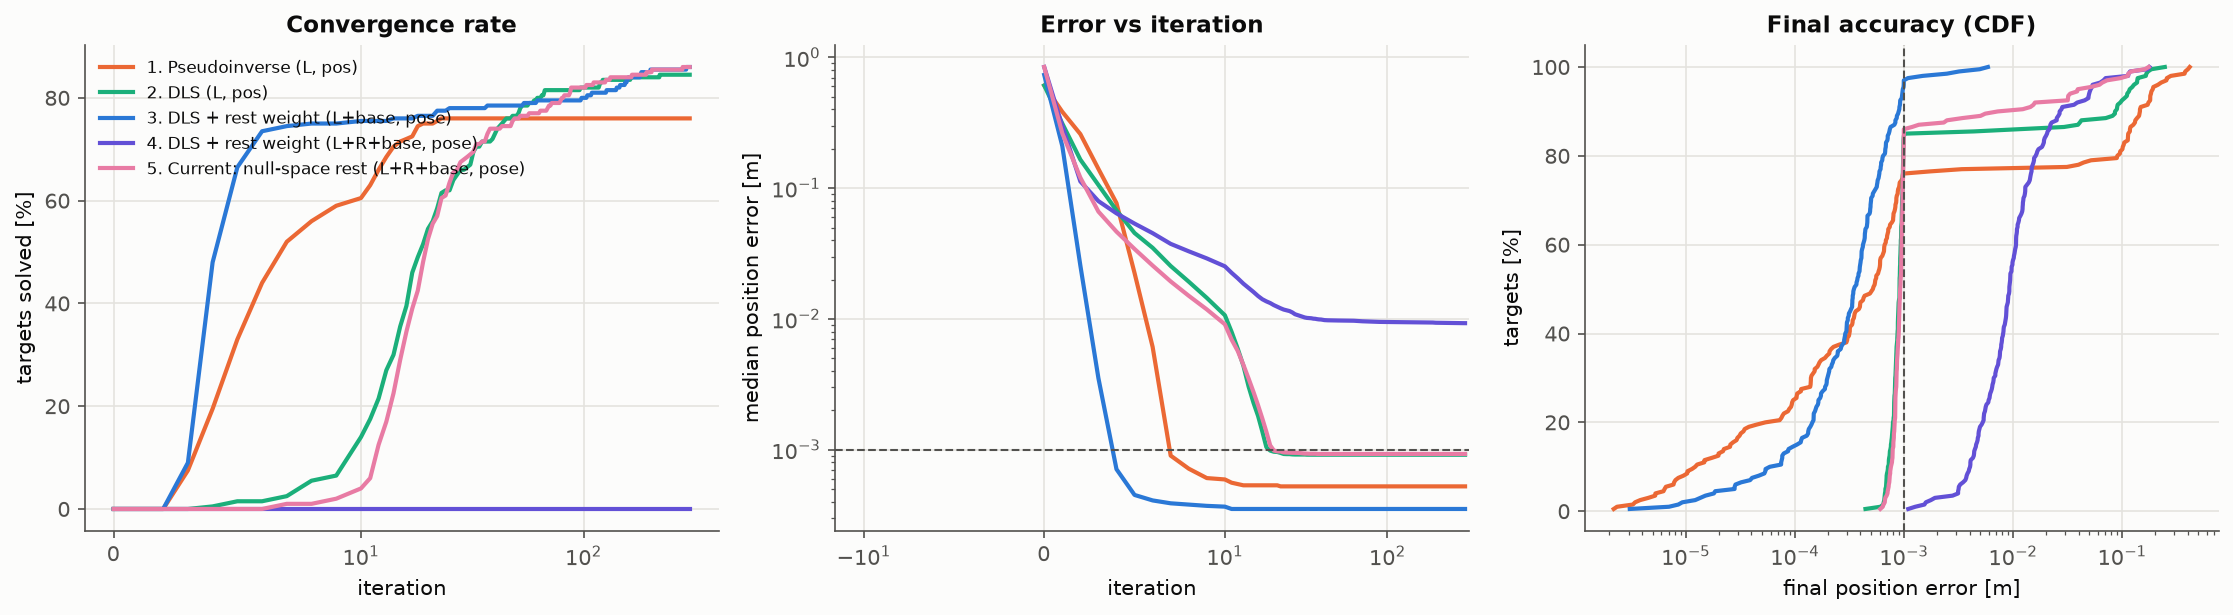
\includegraphics[width=\linewidth]{C_random.png}
    \caption{\small{Experiment C on 200 random targets: share of targets solved against iterations,
    median error against iterations, and distribution of the final error.}}
    \label{fig:bench_c}
\end{figure}

\begin{table}[H]
    \centering
    \footnotesize
    \setlength{\tabcolsep}{3pt}
    \begin{tabular}{lcccccc}
        \toprule
        Stage & Task & Solved & \shortstack{Iter.\\median} & \shortstack{Solve time\\median (ms)} &
        \shortstack{Final pos. error\\median / p95 (mm)} & \shortstack{Largest step\\p95 (rad)} \\
        \midrule
        1. Pseudoinverse & L, pos. & 76.0\,\% & 6 & 0.75 & 0.52 / 191.3 & 4.76 \\
        2. DLS & L, pos. & 84.5\,\% & 17 & 2.23 & 0.91 / 118.0 & 1.52 \\
        3. DLS + rest weight & L + base, pose & 86.0\,\% & 4 & 1.75 & 0.35 / 0.98 & 1.27 \\
        4. DLS + rest weight & L + R + base, pose & 0.0\,\% & -- & -- & 9.27 / 51.7 & 1.61 \\
        5. Null-space rest & L + R + base, pose & 86.0\,\% & 19 & 14.0 & 0.93 / 39.9 & 1.57 \\
        \bottomrule
    \end{tabular}
    \caption{\small{Experiment C summary. For two-hand tasks the error is the larger of the left- and right-hand errors. Each
    run stops at the first iteration below tolerance, so a sub-millimetre median reflects the size of
    the last step, not accuracy. Solve times are for the Python implementation (0.13--0.75\,ms per
    iteration).}}
    \label{tab:bench_c}
\end{table}

The results support the sequence of design decisions. DLS raises the success rate over the
pseudoinverse (84.5 versus 76.0\,\%) and cuts the largest steps by a factor of three, at the cost of
roughly three times as many iterations. With the base available, a single arm reaches pose targets
fastest (median 4 iterations). For two arms, the soft rest weight never reaches the 1\,mm tolerance
(median final error 9.3\,mm), confirming the non-zero equilibrium predicted by
\eqref{eq:rest_normal}, while the null-space formulation reaches 86\,\% of the targets with a median
final error of 0.93\,mm.

Stages 3 and 5 should not be compared directly. Stage 3 tracks one hand (6 rows, 11 joints), while
stage 5 tracks both hands (12 rows, 18 joints) and is scored on the larger of its two hand errors. The difference in
their medians (0.35 versus 0.93\,mm) only reflects convergence speed: every converged run stops at the
first iteration below 1\,mm, and stage 3 gets there in about 4 large steps that overshoot well below
the threshold, while stage 5 takes about 19 smaller damped steps that cross it just under 1\,mm, as
plain DLS does (0.91\,mm). The p95 values differ because the two stages fail differently. The 28
targets that stage 3 misses are orientation-only misses (position essentially exact, orientation about
0.55$^\circ$ against a 0.5$^\circ$ tolerance), so its p95 position error stays under 1\,mm. The 28 that stage
5 misses are genuine two-hand conflicts through the shared base or joint limits (median 32\,mm,
1.8$^\circ$). For two arms, the like-for-like comparison is stage 4 against stage 5: 0 versus 86\,\% of
targets reached.

The null-space formulation's median solve time of 14\,ms is the cost of solving an 18-joint,
12-row system with an SVD-based projector in Python; in the live loop a single iteration (0.75\,ms) is
taken per control cycle, so this is not a bottleneck.

% ============================================================
\section{Integration on the Walkie Simulation}
\label{sec:walkie}

The Walker model was a stand-in: its arms are mounted differently from Walkie's and link 3--4 is
0.154\,m instead of 0.204\,m, so its DH tables do not describe the real robot. This section describes
how the solver was moved onto the full Walkie simulation and how its solutions are executed with the
robot's existing navigation and manipulation stacks (Fig.~\ref{fig:pipeline}). The implementation is
the \texttt{full\_body\_ik} tool in \texttt{walkie-ros}.

\subsection{Kinematic Model from the Robot Description}

Instead of a hand-written DH chain, the forward kinematics and Jacobians are computed by MuJoCo from
the same MJCF model that the simulator runs, which is in turn generated from the real robot's
description. For each hand, the solver queries the hand's tool-centre-point (TCP) pose and its
translational and rotational Jacobians, and keeps the columns of the base, lift and that arm. The base
is the floating joint of \texttt{base\_footprint} restricted to the plane, so its columns are those of
a planar joint:
\begin{equation}
    \mathbf{J}_{v,x}=\hat{\mathbf{x}},\quad
    \mathbf{J}_{v,y}=\hat{\mathbf{y}},\quad
    \mathbf{J}_{v,\psi}=\hat{\mathbf{z}}\times\left(\mathbf{p}_E-\mathbf{p}_B\right),\quad
    \mathbf{J}_{\omega,\psi}=\hat{\mathbf{z}},\quad
    \mathbf{J}_{\omega,x}=\mathbf{J}_{\omega,y}=\mathbf{0},
    \label{eq:planar_base}
\end{equation}
and the lift column is $\mathbf{J}_{v,z_l}=\hat{\mathbf{z}}$. Joint limits (lift 0--0.7435\,m and the arm
ranges) are read from the same model, while the base is unbounded in the solver and constrained by the
map at execution time. The solver itself (Eqs.~\eqref{eq:weighted_dls}--\eqref{eq:nullspace}) was
copied unchanged with the same tuning.

\subsection{Secondary Tasks: Desired Base Pose and Mirrored Rest Posture}

Two changes were made to the desired configuration $\mathbf{q}^{\mathrm{des}}$ in \eqref{eq:nullspace}:
\begin{itemize}
    \item \textbf{Base.} On the Walker model the base was pulled towards the map origin. On Walkie it is
          pulled towards where the robot currently is, $(x,y,\psi)^{\mathrm{des}}=(x,y,\psi)_{\mathrm{now}}$,
          refreshed whenever the solver is synchronised with the robot. The base therefore moves only as
          far as the arms need it to, which is the behaviour wanted for coordinated grasping.
    \item \textbf{Arms.} Both arms are pulled towards a rest posture. The right arm's rest posture is the
          mirror image of the left across the robot's sagittal ($x$--$z$) plane, which for the OpenArm
          kinematics is
          \begin{equation}
              \mathbf{q}_R^{\mathrm{rest}}=\mathbf{S}\,\mathbf{q}_L^{\mathrm{rest}},\qquad
              \mathbf{S}=\operatorname{diag}(-1,-1,-1,1,-1,-1,-1),
          \end{equation}
          with $\mathbf{q}_L^{\mathrm{rest}}=(0,-0.4,0.2,1.7,0.06,0,0)$\,rad (verified with the MJCF forward
          kinematics).
\end{itemize}
Both gains are $K=0.05$ per iteration. To give smooth motion when a target jumps, each step is scaled
so that no joint moves more than $s_{\max}=0.05$ (rad or m) per iteration:
$\Delta\mathbf{q}\leftarrow\Delta\mathbf{q}\cdot\min\!\left(1,\ s_{\max}/\|\Delta\mathbf{q}\|_\infty\right)$.

\subsection{Interactive Tool and Preview}

The IK runs at 100\,Hz on a separate, kinematic-only copy of the robot shown in a MuJoCo preview
window (Fig.~\ref{fig:tool}), so the user sees the expected outcome before anything moves. Targets are
set with sliders (in the map frame or relative to the base) or by dragging them in the preview, and
check boxes choose which base groups (planar position, heading, lift) the solver may use. The preview
is synchronised with the real robot state from \texttt{/joint\_states} and the TF transform
\texttt{map}$\to$\texttt{base\_footprint}, and it can load the same named world as the simulator.
Only when \textbf{Execute} is pressed is the solution sent to the robot.

\begin{figure}[H]
    \centering
    \figplaceholder{0.85\linewidth}{6cm}
    \caption{\small{Full-body IK tool on Walkie: control window and MuJoCo preview with targets, next to
    the simulated robot in the Chulapat~14 world.}}
    \label{fig:tool}
\end{figure}
\pending{Screenshot of the tool (control window + preview + simulator) for Fig.~\ref{fig:tool}, and a
link to a demonstration video.}

\subsection{Execution Through Nav2 and MoveIt}

The IK solution $\mathbf{q}^{*}$ is a goal configuration, not a trajectory: it says where the base,
lift and arms should end, but not how to get there without collisions. Three ways of executing it were
implemented, chosen from the distance $d=\|(x^*,y^*)-(x,y)\|$ between the current and goal base
positions:
\begin{equation}
    \text{execution}(d)=
    \begin{cases}
        \text{lift and arms only (MoveIt hybrid planning)}, & d<1\,\mathrm{cm}\ \text{and}\ |\Delta\psi|<1^\circ,\\
        \text{one whole-body plan (MoveIt)}, & d\le 0.75\,\mathrm{m},\\
        \text{Nav2 approach, then one whole-body plan}, & d>0.75\,\mathrm{m}.
    \end{cases}
    \label{eq:exec_rule}
\end{equation}

\paragraph{Whole-body planning group.}
MoveIt normally plans for the arms and lift with the base fixed. A new planning group
\texttt{whole\_body} adds the base as a planar virtual joint ($x$, $y$, $\theta$) from the
\texttt{map} frame to \texttt{base\_footprint}, so OMPL (RRT-Connect~\cite{kuffner2000}) plans base,
lift and both arms as one 18-dimensional motion and collision-checks the whole robot along it. The
base is sampled only inside a box extending 0.5\,m beyond the start and goal positions. Since the head
camera does not see low obstacles around the base, the occupied cells of the Nav2 map inside that box
are added to the planning scene as boxes 0.05--0.45\,m high before each plan, and the base links are
checked against these boxes; the lift, arms and head are checked against the octomap built from the
head camera. The boxes stop below table height, so the arms can still reach over a table whose legs the
map marks.

\paragraph{Whole-body executor.}
MoveIt can plan the virtual joint but cannot execute it, since no controller owns it. A dedicated
executor runs the trajectory on one clock at 50\,Hz. The base reference
$\mathbf{r}(t)=(x_r,y_r,\psi_r)$ is tracked with feed-forward velocity plus proportional correction,
\begin{equation}
    \mathbf{v}_{\mathrm{map}} = s\,\dot{\mathbf{r}}(t) + \mathbf{K}_p\left(\mathbf{r}(t)-\mathbf{x}_B\right),
    \qquad
    \mathbf{K}_p=\operatorname{diag}(1.5,1.5,1.5)\ \mathrm{s}^{-1},
\end{equation}
limited to 0.5\,m/s and 1\,rad/s, rotated into the base frame and sent as a velocity command. The
arm and lift controllers receive the trajectory point 0.1\,s ahead on the same clock. If the base falls
behind, the clock is slowed so that the arms wait for it:
\begin{equation}
    \dot t = s,\qquad
    s=\operatorname{clip}\!\left(\frac{e_{\mathrm{stop}}-\|\mathbf{r}_{xy}(t)-\mathbf{x}_{B,xy}\|}{e_{\mathrm{stop}}-e_{\mathrm{slow}}},\ 0,\ 1\right),
    \qquad e_{\mathrm{slow}}=0.05\,\mathrm{m},\ e_{\mathrm{stop}}=0.15\,\mathrm{m}.
\end{equation}
The goal succeeds when the base is within 2\,cm and 0.02\,rad of its final pose and every joint within
0.05\,rad. This keeps the hands on the planned path even when the omni base, driven through wheel
contact, lags its reference.

\paragraph{Far goals.}
For base goals beyond 0.75\,m, Nav2 first drives the base to an approach pose 0.5\,m from the goal
with the goal's heading, choosing the closest point on that circle with 0.3\,m of free map around it,
while the arms move to a compact travel pose. The whole-body plan then covers the last part. The
travel pose is the mirrored pose $(0.69,-0.25,0.11,1.92,0,0,-1.57)$, except that the right shoulder
uses $-0.60$\,rad: the exact mirror touches a column on the right side of the base collision model by
2\,mm.

\paragraph{Lift and arms only.}
When the base does not move, the lift and arms go to MoveIt's hybrid planning: a global planner
(OMPL) plans the motion, and a local planner follows it at 10\,Hz and stops the arms if the octomap
shows a new obstacle on the remaining path, after which the global planner replans. Several defects
of the hybrid planning package had to be worked around (an empty start state in the global trajectory,
a combined 15-joint trajectory that the per-arm controllers reject, and a crash after a failed replan).

\begin{figure}[H]
    \centering
    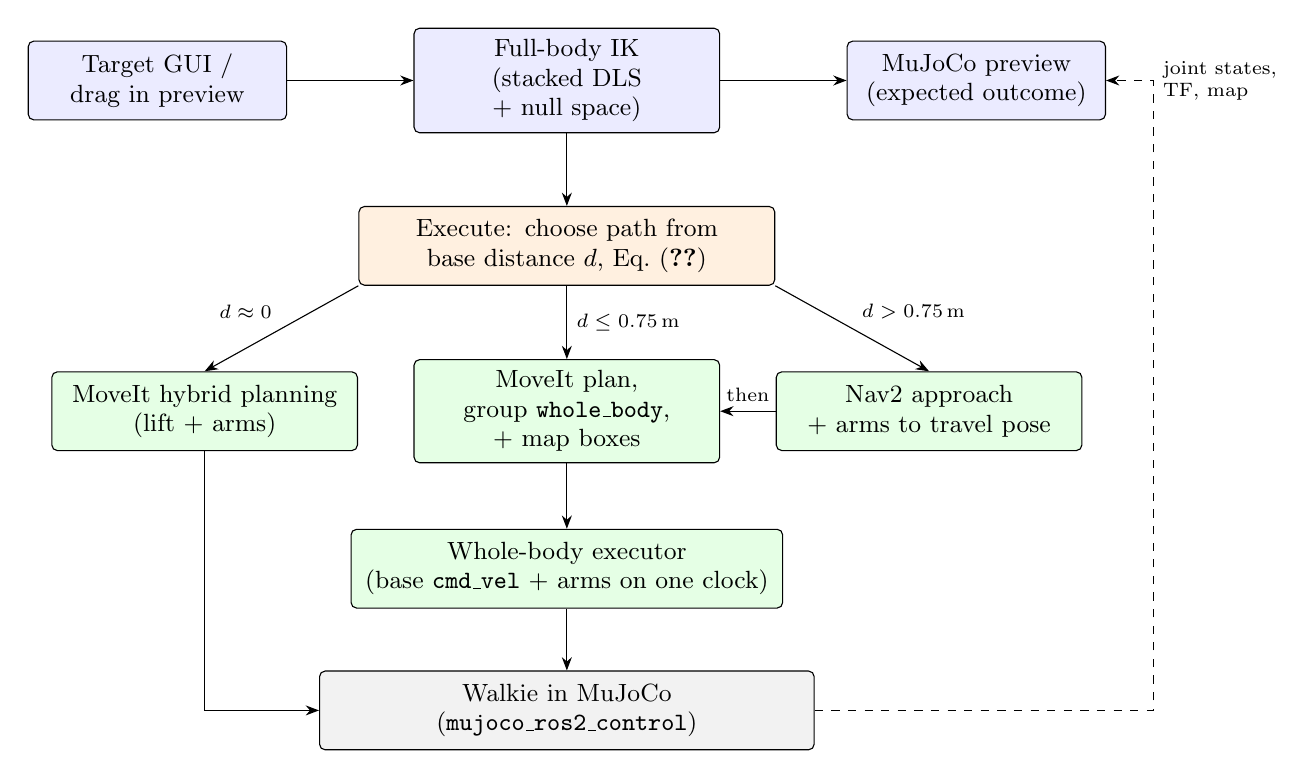
\begin{tikzpicture}[
        >=Stealth, font=\small,
        box/.style={draw, rounded corners=2pt, align=center, minimum height=10mm, text width=#1, inner sep=4pt,
                    execute at begin node=\setlength{\baselineskip}{1.15em}},
        box/.default=3.6cm]
        \node[box=3.6cm, fill=blue!8] (ik) at (0,0) {Full-body IK\\(stacked DLS + null space)};
        \node[box=3.0cm, fill=blue!8] (gui) at (-5.2,0) {Target GUI /\\drag in preview};
        \node[box=3.0cm, fill=blue!8] (prev) at (5.2,0) {MuJoCo preview\\(expected outcome)};
        \node[box=5.0cm, fill=orange!12] (dec) at (0,-2.1) {Execute: choose path from\\base distance $d$, Eq.~(\ref{eq:exec_rule})};
        \node[box, fill=green!10] (hyb) at (-4.6,-4.2) {MoveIt hybrid planning\\(lift + arms)};
        \node[box, fill=green!10] (wb) at (0,-4.2) {MoveIt plan, group \texttt{whole\_body}, + map boxes};
        \node[box, fill=green!10] (nav) at (4.6,-4.2) {Nav2 approach\\+ arms to travel pose};
        \node[box=5.2cm, fill=green!10] (exe) at (0,-6.2) {Whole-body executor\\(base \texttt{cmd\_vel} + arms on one clock)};
        \node[box=6.0cm, fill=gray!10] (sim) at (0,-8.0) {Walkie in MuJoCo (\texttt{mujoco\_ros2\_control})};
        \draw[->] (gui) -- (ik);
        \draw[->] (ik) -- (prev);
        \draw[->] (ik) -- (dec);
        \draw[->] (dec.south west) -- node[above left, font=\scriptsize]{$d\approx0$} (hyb.north);
        \draw[->] (dec) -- node[right, font=\scriptsize]{$d\le0.75$\,m} (wb);
        \draw[->] (dec.south east) -- node[above right, font=\scriptsize]{$d>0.75$\,m} (nav.north);
        \draw[->] (nav) -- node[above, font=\scriptsize]{then} (wb);
        \draw[->] (wb) -- (exe);
        \draw[->] (exe) -- (sim);
        \draw[->] (hyb) |- (sim);
        \draw[->, dashed] (sim.east) -| ([xshift=6mm]prev.east) |- node[pos=0.25, right, font=\scriptsize, align=left]{joint states,\\TF, map} (prev.east);
    \end{tikzpicture}
    \caption{\small{Integration of the full-body IK with MoveIt and Nav2 on the Walkie simulation.}}
    \label{fig:pipeline}
\end{figure}

\subsection{Known Limitations}

\begin{itemize}
    \item The IK has no collision model; collisions are handled only by MoveIt when the solution is
          planned. A goal configuration that overlaps an obstacle or itself is rejected at that stage.
    \item The simulated head camera's depth reads about 15\,\% short, so the octomap places the floor at
          about $z=0.17$\,m and obstacles closer than they are. This is why the base links are checked
          against the Nav2 map instead of the octomap. Phantom voxels can block later plans until the
          octomap is cleared.
    \item After a whole-body goal, AMCL's next update can shift the base by a few centimetres (up to
          about 10\,cm observed) in the map frame, moving the hands by the same amount. Executing again
          corrects it.
\end{itemize}

% ============================================================
\section{Simulation Evaluation of Whole-Body Execution}
\label{sec:exec_eval}

\subsection{Method}

A benchmark (\texttt{full\_body\_ik/benchmark\_execution.py} in \texttt{walkie-ros}) measures how well
whole-body execution reproduces the IK solution on the simulated robot. Each trial samples a two-hand
6D target that requires the base to move: the hand poses of a virtual robot whose base is displaced
0.25--0.6\,m from the current pose (heading within $\pm90^\circ$ of the robot's, yaw change within
$\pm0.5$\,rad), with the lift changed by up to 0.15\,m and each arm joint perturbed by up to 0.3\,rad
around the rest posture. The IK is iterated from the robot's state, as the tool does, until both hands
are within 1\,mm and 0.01\,rad, and the solution is executed with a whole-body plan. One second after
the executor reports completion, the hand errors to the targets and the base error to the IK base pose
are measured from \texttt{/joint\_states} and TF with the MJCF forward kinematics. Before each trial,
the arms and lift are returned to the home pose. Times are in simulation time. The trials run in the
empty world with odometry localisation, so that AMCL corrections do not affect the measurement.
Per-trial results are listed in Appendix~\ref{app:exec_trials}.

\subsection{Results}

% Numbers from walkie-ros/full_body_ik/results/execution_runs.csv (mode whole_body)
\begin{table}[H]
    \centering
    \small
    \begin{tabular}{lccc}
        \toprule
        Quantity & Median & Min & Max \\
        \midrule
        Execution time (s) & 8.2 & 4.1 & 14.5 \\
        Hand position error, max of both hands (mm) & 12.0 & 10.8 & 13.8 \\
        Hand orientation error, max of both hands ($^\circ$) & 1.40 & 1.33 & 1.50 \\
        Base position error (mm) & 0.9 & 0.2 & 1.7 \\
        Base heading error ($^\circ$) & 0.03 & 0.01 & 0.07 \\
        \bottomrule
    \end{tabular}
    \caption{\small{Whole-body execution of 15 IK solutions with base goals 0.18--0.55\,m away (empty
    world). All 15 executions succeeded. Hand errors are the larger of the left- and right-hand errors
    in each trial.}}
    \label{tab:exec}
\end{table}

\begin{figure}[H]
    \centering
    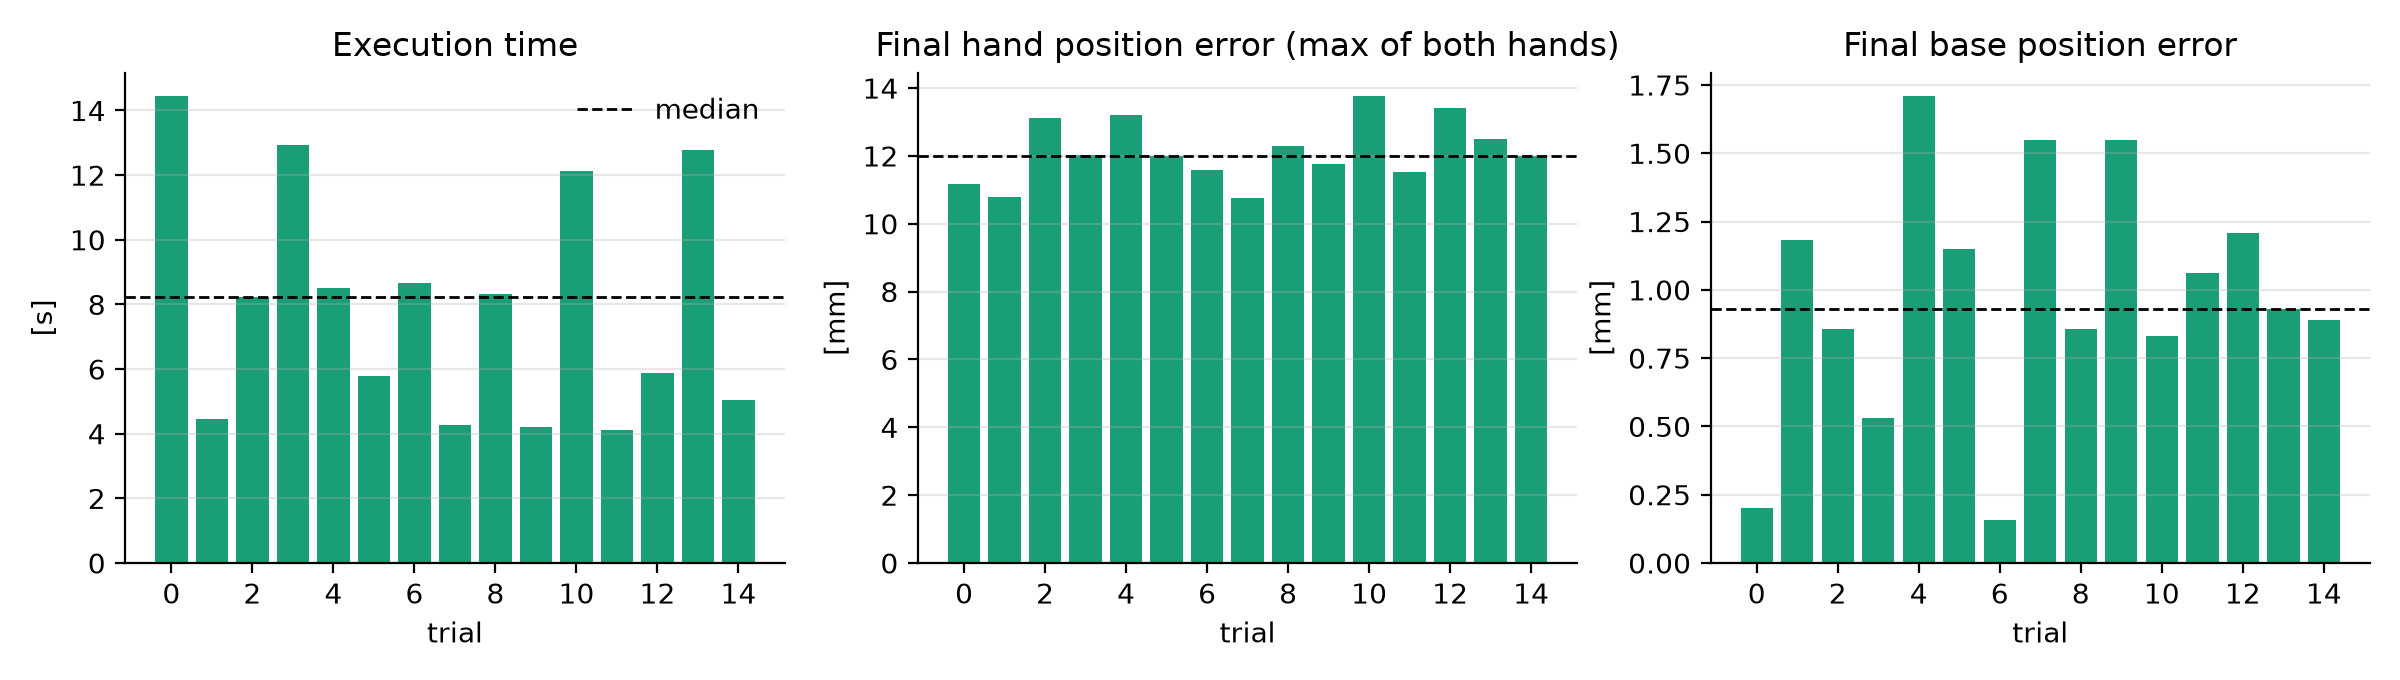
\includegraphics[width=\linewidth]{execution_benchmark.png}
    \caption{\small{Whole-body execution per trial: execution time, final hand position error and final
    base position error.}}
    \label{fig:exec}
\end{figure}

All 15 solutions were executed successfully, with a median execution time of 8.2\,s. The base ended
within 1.7\,mm and 0.07$^\circ$ of the IK base pose, well inside the executor's 2\,cm tolerance, because the
executor tracks the planned base trajectory with feed-forward and feedback and holds the arms back
whenever the base lags. The hands ended 10.8--13.8\,mm and about 1.4$^\circ$ from their targets. Since the
base error is below 2\,mm, this residual comes from the arms: it is consistent with the steady-state
error of the MuJoCo arm position controllers (about 0.01\,rad per joint, which the executor's 0.05\,rad
joint tolerance accepts) acting over the length of the arm. Reducing it is a controller-tuning task
rather than a planning one. The narrow spread of the hand error across trials (3\,mm) shows that it does
not depend on how far the base had to move.

These results are limited to an empty world and 15 trials, with base goals inside the 0.75\,m
whole-body radius.

\pending{Repeat the benchmark in the Chulapat~14 world (AMCL, furniture) and with goals beyond the
0.75\,m whole-body radius, where the Nav2 approach is used.}

% ============================================================
\section{Path Planning (In Progress)}
\label{sec:planning}

The whole-body plan of Section~\ref{sec:walkie} is limited to a box around the start and goal and
uses MoveIt's default RRT-Connect without modification. Longer motions through cluttered rooms,
narrow passages between furniture, and the choice of the base pose itself are the subject of the
current work. This section summarises the methods under investigation and how they relate to Walkie.

\subsection{Problem Definition}

Let $\mathcal{C}\subset\mathbb{R}^{18}$ be the configuration space of \eqref{eq:q18},
$\mathcal{C}_{obs}$ the configurations in collision and
$\mathcal{C}_{free}=\mathcal{C}\setminus\mathcal{C}_{obs}$. A feasible path is a continuous
$\sigma:[0,1]\to\mathcal{C}_{free}$ with $\sigma(0)=\mathbf{q}_{init}$ and
$\sigma(1)\in\mathcal{C}_{goal}$~\cite{chai2022}. An optimal path additionally minimises a cost
$c(\sigma)$ over all feasible paths. For grasping, the goal is not one configuration but the set of
all configurations that place the hands at the grasp poses,
\begin{equation}
    \mathcal{C}_{goal}=\left\{\mathbf{q}\in\mathcal{C}_{free}\ :\ {}^{W}\mathbf{T}_{E_k}(\mathbf{q})={}^{W}\mathbf{T}_{k}^{\mathrm{grasp}},\ k\in\{L,R\}\right\},
\end{equation}
a 6- to 12-dimensional manifold for the redundancies of Table~\ref{tab:modes}. Committing to one IK
solution, as the current pipeline does, discards most of this goal set~\cite{vahrenkamp2010}.

\subsection{RRT and RRT-Connect}

RRT grows a tree $\mathcal{T}$ from $\mathbf{q}_{init}$. Each iteration samples
$\mathbf{q}_{rand}$, finds the nearest vertex $\mathbf{q}_{near}$ under a metric $\rho$, and steps a
fixed distance $\epsilon$ towards the sample:
\begin{equation}
    \mathbf{q}_{new}=\mathbf{q}_{near}+\min\!\left(\epsilon,\ \rho(\mathbf{q}_{near},\mathbf{q}_{rand})\right)
    \frac{\mathbf{q}_{rand}-\mathbf{q}_{near}}{\|\mathbf{q}_{rand}-\mathbf{q}_{near}\|}.
\end{equation}
If the segment is collision-free, $\mathbf{q}_{new}$ is added (\emph{Advanced}, or \emph{Reached} if it
equals the sample); otherwise the step is \emph{Trapped}. Because a vertex is selected with probability
proportional to the volume of its Voronoi region, the tree is biased towards unexplored space, and its
vertex distribution converges to the sampling distribution, which makes RRT probabilistically
complete~\cite{kuffner2000}. RRT-Connect (Algorithm~\ref{alg:rrtconnect}) grows two trees, from the
start and from the goal, and after each extension repeatedly extends the other tree towards the new
vertex (\textsc{Connect}) until it is reached or blocked; a long path then costs a single
nearest-neighbour query. The greedy connection works best in relatively open spaces and was originally
developed for 7-DOF arm grasping~\cite{kuffner2000}.

\begin{algorithm}[H]
\caption{RRT-Connect~\cite{kuffner2000}}
\label{alg:rrtconnect}
\begin{algorithmic}[1]
\Function{Connect}{$\mathcal{T}, \mathbf{q}$}
    \Repeat \ $S\gets$ \Call{Extend}{$\mathcal{T},\mathbf{q}$}
    \Until{$S\neq$ \emph{Advanced}}
    \State \Return $S$
\EndFunction
\Function{RRT-Connect}{$\mathbf{q}_{init},\mathbf{q}_{goal}$}
    \State $\mathcal{T}_a\gets\{\mathbf{q}_{init}\}$, \ $\mathcal{T}_b\gets\{\mathbf{q}_{goal}\}$
    \For{$k=1$ \textbf{to} $K$}
        \State $\mathbf{q}_{rand}\gets$ \Call{RandomConfig}{}
        \If{\Call{Extend}{$\mathcal{T}_a,\mathbf{q}_{rand}$} $\neq$ \emph{Trapped}}
            \If{\Call{Connect}{$\mathcal{T}_b,\mathbf{q}_{new}$} $=$ \emph{Reached}}
                \State \Return \Call{Path}{$\mathcal{T}_a,\mathcal{T}_b$}
            \EndIf
        \EndIf
        \State \Call{Swap}{$\mathcal{T}_a,\mathcal{T}_b$}
    \EndFor
    \State \Return \emph{Failure}
\EndFunction
\end{algorithmic}
\end{algorithm}

\subsection{Optimality and Sampling Strategies: RRT* and Its Variants}

RRT* chooses for each new vertex the parent that minimises the cost-to-come within a neighbourhood
and rewires neighbours through the new vertex when that lowers their cost, which makes it
asymptotically optimal~\cite{hameed2025}. Its practical weaknesses are slow convergence in
high-dimensional or cluttered spaces, neglect of dynamics, collision-checking cost, and the
static-world assumption~\cite{hameed2025}. Three remedies are directly relevant to Walkie:
\begin{itemize}
    \item \textbf{Informed sampling.} Once a solution of cost $C_{\max}$ is known, only states that could
          improve it are sampled, i.e.\ the prolate hyperspheroid
          \begin{equation}
              \|\mathbf{q}-\mathbf{q}_{init}\|+\|\mathbf{q}-\mathbf{q}_{goal}\|\le C_{\max},
          \end{equation}
          which focuses effort without adding tuning parameters~\cite{hameed2025}.
    \item \textbf{Bridge-test sampling.} With probability $P_{BTS}\in[0.1,0.3]$, two configurations
          $\mathbf{p}_1,\mathbf{p}_2$ are drawn; if both collide but their midpoint
          $\mathbf{m}=\tfrac12(\mathbf{p}_1+\mathbf{p}_2)$ is free, $\mathbf{m}$ is used as the sample.
          This places samples inside narrow passages, such as a gap between a table and a chair, while the
          remaining uniform samples preserve coverage~\cite{hameed2025}.
    \item \textbf{Lazy and dynamic variants.} Lazy collision checking defers checks to the edges of a
          candidate path, and dynamic variants (DRRT, RRT$^{\text{X}}$, hybrid RRT*/D* Lite) repair the
          affected part of the tree when obstacles move instead of replanning from
          scratch~\cite{hameed2025}.
\end{itemize}
The survey also notes that most kinodynamic and re-planning methods target low-DOF mobile robots and
that scaling them to 7--10-DOF arms remains largely unexplored~\cite{hameed2025}, which is the
situation of a mobile bimanual robot.

\subsection{Narrow Passages: RJ-RRT}

RJ-RRT~\cite{chai2022} adds two mechanisms to RRT. First, a greedy reduction of the sampling space:
after each successful extension, sampling is restricted to the sub-box between the new vertex and the
goal, and when extension fails, sampling falls back to the gap regions
$\mathrm{Gap}=\mathrm{Original}\setminus(\mathrm{Original}\cap\mathrm{Next})$ recorded at earlier
reductions. Second, an environment judgment: a sample in collision is probed with $N_1$ local samples
within radius $R_1$; if some are free, eight marker points on a circle of radius $R_2$ around a free
sample classify it as inside a narrow passage (two or four free markers in opposite pairs) or at its
entrance, and a sub-tree is grown in a rectangle aligned with the passage and later merged into the main
tree. In 2D benchmarks it reduced planning time by 87\,\% compared with RRT in a cluttered map and by
45\,\% compared with RRV in a narrow passage, with far fewer nodes~\cite{chai2022}. Its performance
depends on the step size, and it has so far been shown only in 2D, so its marker-based judgment would
have to be adapted to the base's planar subspace (where furniture creates the narrow passages) rather
than the full 18-dimensional space.

\subsection{Sampling Goals and Base Positions: IK-RRT}

The IK-RRT of Vahrenkamp et al.~\cite{vahrenkamp2010} is the closest existing method to this project.
A bidirectional RRT starts with the forward tree at the start configuration and an \emph{empty}
backward tree. With probability $p_{IK}$ per iteration (0.03 in their experiments), a randomised IK
solver produces a new goal configuration, including the base position, which is added as a new root
of the backward tree. Planning therefore searches the whole goal set $\mathcal{C}_{goal}$ instead of a
single IK solution. Base positions are sampled from an inverse reachability map built from a
discretised 6D reachability distribution of the arm; for two arms, the bimanual map is the cell-wise
minimum of the two,
\begin{equation}
    R_{bi}(x,y)=\min\!\left(R_{left}(x,y),\ R_{right}(x,y)\right),
\end{equation}
since a bimanual IK solution fails if either arm fails~\cite{vahrenkamp2010}. They planned 20-DOF
bimanual grasps for ARMAR-III in under 10\,s. For Walkie, the stacked null-space IK of
Section~\ref{sec:ik} can serve as the goal sampler: seeding it with different base poses yields
different members of $\mathcal{C}_{goal}$, and its null-space base pull can bias them towards the
current base position.

\subsection{Dynamic Environments: RAMP}

RAMP~\cite{vannoy2008} plans for mobile manipulators among obstacles with unknown motion. It keeps a
population of complete trajectories, each a pair of \emph{loosely coupled} base and arm
sub-trajectories that may pause independently, and continuously improves them with random
modification operators (insert, delete, change, swap, crossover, stop) while the robot executes the
current best one. Feasible trajectories are ranked by
\begin{equation}
    \mathrm{Cost}=C_1\frac{E}{a_1}+C_2\frac{T}{a_2}+C_3\frac{M}{a_3},
\end{equation}
combining energy $E$, time $T$ and an inverse-manipulability term $M$ with weights $C_i$ and
normalisations $a_i$, and infeasible ones by $\mathrm{Cost}+Q/T_{coll}$, which prefers trajectories
whose first predicted collision is later. Allowing the base or arm to stop reduced energy by about
30\,\% at the same execution time, and keeping sub-populations with different departure directions
reduced forced stops~\cite{vannoy2008}. Its cost function is a candidate for
ranking candidate base poses and grasps.

\subsection{Next Step}

The variants above are the methods under review; they address different weaknesses of the basic RRT
(path quality, narrow passages, the choice of goal configuration, moving obstacles). Only one of them
will be implemented, as a replacement for or an extension of the RRT-Connect planner currently used
for the whole-body plan of Section~\ref{sec:walkie}. The choice will be based on which weakness
limits Walkie most in the furnished room.

\pending{The selected method, its implementation and its results.}

% ============================================================
\section{Example Scenarios: Agent Reasoning over Traditional Skills}
\label{sec:skills}

This section illustrates, without results, how the agent is intended to reason about general tasks
once the manipulation skills are available as tools. The agent only decides \emph{what} to do and in
which order; every motion is planned and executed by the traditional control stack, which reports
success or an explicit failure back to the agent. The traces below are illustrative, written in the
form of the agent's tool calls; this part is still in development.

\newcommand{\trace}[2]{%
  \par\smallskip\noindent\fbox{\begin{minipage}{0.95\linewidth}\small
  \textbf{Request:} ``#1''\par\smallskip\ttfamily\footnotesize #2\end{minipage}}\par\medskip}

\paragraph{Pick and place.}
The agent breaks the request into finding the object, going to it, grasping it, going to the person
and handing it over. If a grasp is unreachable, it asks the control stack to move closer or try
another grasp before giving up.
\trace{Bring me the cup from the kitchen.}{%
1.\ find\_object("cup") $\rightarrow$ last seen: kitchen counter\\
2.\ navigate("kitchen counter") $\rightarrow$ succeeded\\
3.\ detect("cup") $\rightarrow$ pose found\\
4.\ pick("cup") $\rightarrow$ failed: unreachable\\
5.\ \textit{reason: the cup is at the back of the counter; approach from the other side}\\
6.\ navigate("kitchen counter", side="left") $\rightarrow$ succeeded\\
7.\ pick("cup") $\rightarrow$ succeeded, grasp detected\\
8.\ navigate("user") $\rightarrow$ succeeded\\
9.\ hand\_over() $\rightarrow$ succeeded; say("Here is your cup.")}

\paragraph{Pointing.}
Pointing needs no grasp: the agent resolves which object or person is meant, and the control stack
turns the base and one arm so the hand points at it.
\trace{Which one is my bag? Point at it.}{%
1.\ find\_object("bag", owner="user") $\rightarrow$ black backpack, living room\\
2.\ detect("black backpack") $\rightarrow$ pose found, 2.1 m away\\
3.\ point("black backpack") $\rightarrow$ succeeded\\
4.\ say("This black backpack next to the sofa is yours.")}

\paragraph{Carrying a bag.}
The agent combines a grasp, a carrying posture and navigation, and releases the bag at the
destination.
\trace{Carry this bag to the entrance.}{%
1.\ detect("bag") $\rightarrow$ handle pose found\\
2.\ pick("bag", grasp="handle, from above") $\rightarrow$ succeeded\\
3.\ carry\_pose() $\rightarrow$ arm close to the body, lift lowered\\
4.\ navigate("entrance") $\rightarrow$ succeeded\\
5.\ place("floor") $\rightarrow$ succeeded; say("I left the bag at the entrance.")}

In each case, the agent's choices are discrete and checkable (which object, which place, which skill
next), while the continuous problems of where the base should stop, how the arms should move and
whether the motion is collision-free stay in the whole-body planner of Section~\ref{sec:walkie}. A
task such as folding laundry does not reduce to a few such calls, which is why it is routed to the
VLA branch instead.

% ============================================================
\section{Real-Robot Experiments}
\label{sec:real}

The software stack used in simulation is the same as on the robot: the same robot description,
ros2\_control controllers, MoveIt configuration and Nav2 parameters. The planned validation follows the
progression of the proposal: known targets on the real robot, then perception-based targets, then
the full task skills called by the agent.
\pending{Real-robot results: base and hand tracking error of whole-body execution, grasp success on the test object set, and the observed
sim-to-real differences (localisation, lift speed of about 3\,cm/s, arm controller gains).}

\begin{figure}[H]
    \centering
    \figplaceholder{0.8\linewidth}{5cm}
    \caption{\small{Whole-body grasping on the real Walkie (placeholder).}}
    \label{fig:real}
\end{figure}

% ============================================================
\section{Vision-Language-Action Branch}
\label{sec:vla}

\tbc

% ============================================================
\section{Discussion of Outcomes So Far}
\label{sec:discussion}

\begin{table}[H]
    \centering
    \small
    \renewcommand{\arraystretch}{1.15}
    \begin{tabular}{p{0.30\linewidth} p{0.36\linewidth} p{0.24\linewidth}}
        \toprule
        Objective & Status & Evidence \\
        \midrule
        1. Unified kinematic model & Done: 18-DOF model from the robot description, FK and Jacobians from
            MuJoCo & Sections~\ref{sec:platform}, \ref{sec:walkie} \\
        2. Coordinated base--arm planning and execution & Whole-body IK done; whole-body planning and
            execution done in simulation; obstacle-rich path planning in progress &
            Sections~\ref{sec:ik}--\ref{sec:planning} \\
        3. General task skills for the agent & Agent with navigation tools done; pick, place, point and carry
            skills designed, in progress & Sections~\ref{sec:arch}, \ref{sec:skills} \\
        4. VLA branch & \multicolumn{2}{l}{\tbcinline} \\
        5. Evaluation in simulation and on the robot & IK benchmarks (200 targets); execution benchmark in
            the empty world; room, skill and real-robot evaluation pending &
            Sections~\ref{sec:ik_bench}, \ref{sec:exec_eval} \\
        6. Task characteristics per branch & Routing criteria defined; to be validated &
            Section~\ref{sec:arch} \\
        \bottomrule
    \end{tabular}
    \caption{\small{Status of the objectives at the time of this draft.}}
    \label{tab:status}
\end{table}

\paragraph{What worked.}
The most important design decision was to treat the base and the arm posture as secondary tasks in the
null space of the hand targets rather than as weights in the same cost. This was the only formulation
that reached two-arm targets while keeping a reasonable posture, and it carried over to Walkie without
change, apart from pulling the base towards its current pose. Computing kinematics from the robot's own
description, rather than a hand-written DH table, removed a whole class of model errors and allowed the
same code to run on the full robot. On the execution side, planning the base and arms as one
collision-checked trajectory and executing it on one clock turned the IK solution into coordinated
motion with base errors of millimetres.

\paragraph{What did not.}
The IK itself is local and collision-unaware, so it can
propose goals that MoveIt then rejects, and a single IK goal ignores the rest of the goal set.

\paragraph{Remaining work.}
The remaining traditional-control work is the path-planning layer (Section~\ref{sec:planning}), the
general task skills and their exposure to the agent (Section~\ref{sec:skills}), and evaluation in the furnished
room and on the real robot. Integrating the VLA branch behind the same agent completes the
architecture.

% ============================================================
\section{Conclusion}

This draft reports a hybrid control architecture for the Walkie mobile manipulator, in which a
language-model agent routes general-purpose tasks to traditional coordinated base--arm control and
hard-to-model tasks to a VLA policy. For the traditional branch, a whole-body IK solver was developed
from the pseudoinverse to a stacked damped least-squares solve with joint-limit damping and null-space
posture and base tasks, validated on 200 random targets, and transferred to the full Walkie simulation
with kinematics taken from the robot description. Its solutions are executed as a single whole-body
MoveIt plan with a dedicated executor, which in simulation executed every test solution with the
base within 2\,mm and the hands within 14\,mm of their targets. Path planning with sampling-based methods, the general task
skills exposed to the agent, real-robot validation and the VLA branch are in progress and will be
added to the final report.

\clearpage
\bibliography{citations}

% ============================================================
% APPENDICES (included from main.tex after the bibliography)
% ============================================================
\clearpage
\appendix
\renewcommand{\thesection}{\Alph{section}}

\section{Videos}
\label{app:videos}

\begin{table}[H]
    \centering
    \small
    \renewcommand{\arraystretch}{1.2}
    \begin{tabular}{p{0.06\linewidth} p{0.56\linewidth} p{0.30\linewidth}}
        \toprule
        No. & Content & Link \\
        \midrule
        V1 & Unified base--arm model: OpenArm with virtual base joints in MuJoCo (first progress report) &
            \vidlink{https://youtu.be/VUVee6bROx8}{youtu.be/VUVee6bROx8} \\
        V2 & Pseudoinverse versus DLS near a singular configuration (Fig.~\ref{fig:singularity}) &
            \vidlink{https://youtu.be/MEW62I4-9JQ}{youtu.be/MEW62I4-9JQ} \\
        V3 & Single arm: per-joint DLS versus DLS with the rest pull (Fig.~\ref{fig:rest_single}) &
            \vidlink{https://youtu.be/wrWfXNqLJrA}{youtu.be/wrWfXNqLJrA} \\
        V4 & Two arms: averaged base step versus stacked solve on the showcase target pair
            (Table~\ref{tab:app_showcase}) & \vidlink{https://youtu.be/Ey7bL1Zsx1M}{youtu.be/Ey7bL1Zsx1M} \\
        V5 & Live full-body IK with the mode GUI (hands, orientation, base and lift) &
            \vidlink{https://youtu.be/Kn5jznpRHcw}{youtu.be/Kn5jznpRHcw} \\
        V6 & Weighted rest pose, no posture term and null-space rest posture on the benchmark targets
            (Fig.~\ref{fig:nullspace}) & \vidlink{https://youtu.be/3rgqf_vf3_w}{youtu.be/3rgqf\_vf3\_w} \\
        V7 & Full-body IK tool on the Walkie simulation: preview and whole-body execution & \tbcinline \\
        \bottomrule
    \end{tabular}
    \caption{\small{Videos referenced in this report.}}
    \label{tab:videos}
\end{table}

\section{Software and Reproduction}
\label{app:software}

\begin{table}[H]
    \centering
    \small
    \renewcommand{\arraystretch}{1.2}
    \begin{tabular}{p{0.33\linewidth} p{0.60\linewidth}}
        \toprule
        Repository & Contents \\
        \midrule
        \vidlink{https://github.com/MonochromePie/Coordinated-Base-Arm-Motion-Control}{Coordinated-Base-Arm-Motion-Control}
            & IK solver and its versions (\texttt{walker\_robot/}), offline benchmark (\texttt{benchmark/}),
              scenario playback (\texttt{ik\_sim/}), Walker MuJoCo models, and these reports (\texttt{report/}) \\
        \vidlink{https://github.com/EIC-Robocup-2026/walkie-ros}{walkie-ros}
            & Walkie robot software: description and MuJoCo model, Nav2, MoveIt configuration with the
              \texttt{whole\_body} group and executor, named worlds, and the full-body IK tool and
              execution benchmark (\texttt{full\_body\_ik/}). Branch \texttt{feat/moveit-full-body}
              (\texttt{1da4535}) adds the commander's whole-body goals and the launch file and guide
              for the real robot; \texttt{feat/sim-bottle-pick} (\texttt{e31c1bf}) builds on it and
              adds the scripted bottle pick \\
        \vidlink{https://github.com/EIC-Robocup-2026/walkie-agent-ros}{walkie-agent-ros}
            & Task-level agent: typed tools including \texttt{pick\_object}, voice input and output,
              the simulation oracle for people, and the runbook for the real robot. Branch
              \texttt{feat/mahoraga-demo} (\texttt{dd49c1d}) \\
        \vidlink{https://github.com/EIC-Robocup-2026/walkie-vision}{walkie-vision}
            & Perception from the head camera: people, and open-vocabulary objects with YOLOE. Branch
              \texttt{feat/scene-graph-prep} (\texttt{ad7c833}) \\
        \vidlink{https://github.com/EIC-Robocup-2026/walkie-database}{walkie-database}
            & Memory of people and of perceived objects, read by the agent. Branch
              \texttt{feat/scene-graph-prep} (\texttt{41dae92}) \\
        \bottomrule
    \end{tabular}
    \caption{\small{Code repositories.}}
    \label{tab:app_repos}
\end{table}

\paragraph{Offline IK benchmark (Section~\ref{sec:ik_bench}).} From the root of Coordinated-Base-Arm-Motion-Control:
\begin{verbatim}
uv sync
uv run benchmark/run_benchmark.py    # experiments A, B, C
uv run ik_sim/run_ik_sim.py B --record    # playback + keyframes
\end{verbatim}

\paragraph{Execution benchmark (Section~\ref{sec:exec_eval}).} From the root of walkie-ros, each command
in its own terminal:
\begin{verbatim}
pixi run ros2 run rmw_zenoh_cpp rmw_zenohd
pixi run ros2 launch robot_bringup nav_mujoco_omnibot.launch.py headless:=true
pixi run ros2 launch openarm_bimanual_moveit_config moveit_only.launch.py \
    hardware_type:=mujoco
pixi run python -u full_body_ik/benchmark_execution.py --trials 15 --seed 1 \
    --out full_body_ik/results
\end{verbatim}
The figure and the table rows are regenerated from the results with:
\begin{verbatim}
uv run report/final_draft/scripts/plot_execution.py \
    ~/walkie-ros/full_body_ik/results/execution_runs.csv
\end{verbatim}

\paragraph{Interactive full-body IK tool (Section~\ref{sec:walkie}).} With the simulation and MoveIt
running as above:
\begin{verbatim}
pixi run python full_body_ik/run_full_body_ik.py [--world chula_pat14_6]
\end{verbatim}

\paragraph{Whole-body goals in the commander (Section~\ref{sec:commander_results}).} From the root of
walkie-ros on branch \texttt{feat/sim-bottle-pick}, each command in its own terminal:
\begin{verbatim}
pixi run ros2 launch robot_bringup whole_body_demo.launch.py
pixi run ros2 run openarm_bimanual_commander_cpp whole_body_demo
\end{verbatim}
The launch file starts the test scene, Nav2 (which owns the collision monitor), \texttt{move\_group},
the commander, the base follower, RViz and a Zenoh router. \texttt{headless:=true} with
\texttt{use\_rviz:=false} runs it without windows, and \texttt{start\_router:=false} uses a router that is already running. The
demo client takes \texttt{--cycles} \textit{N} for repeated round trips and \texttt{--report}
\textit{file} to write its report to a file.

\paragraph{Scripted bottle pick (Section~\ref{sec:pick}).} From the same checkout, on a Zenoh router
and ROS domain of its own (port 7511 and domain 81 are an example). The router, in a first terminal:
\begin{verbatim}
export ROS_DOMAIN_ID=81
unset ZENOH_ROUTER_CONFIG_URI ZENOH_SESSION_CONFIG_URI
export ZENOH_CONFIG_OVERRIDE=\
'listen/endpoints=["tcp/localhost:7511"];connect/endpoints=[]'
pixi run ros2 run rmw_zenoh_cpp rmw_zenohd
\end{verbatim}
First in each of two further terminals:
\begin{verbatim}
export ROS_DOMAIN_ID=81
unset ZENOH_ROUTER_CONFIG_URI ZENOH_SESSION_CONFIG_URI
export ZENOH_CONFIG_OVERRIDE='connect/endpoints=["tcp/localhost:7511"]'
\end{verbatim}
then the simulation in one and the pick in the other:
\begin{verbatim}
pixi run ros2 launch robot_bringup whole_body_demo.launch.py \
    world:=chula_pat14_6 start_router:=false
pixi run ros2 run robot_bringup sim_bottle_pick.py \
    --report /tmp/pick.json
\end{verbatim}
The pick runs once per launch; restart the launch to put the bottle back on the table.

\section{Denavit--Hartenberg Parameters of the Walker Model}
\label{app:dh}

\begin{table}[H]
    \centering
    \small
    \begin{tabular}{ccccc}
        \toprule
        Link & $d$ (m) & $\theta$ (rad) & $a$ (m) & $\alpha$ (rad) \\
        \midrule
        1  & 0 & $-\pi/2$ & 0 & $-\pi/2$ \\
        2  & $x^*$ & 0 & 0 & 0 \\
        3  & 0 & 0 & 0 & $\pi/2$ \\
        4  & 0 & $\pi/2$ & 0 & $-\pi/2$ \\
        5  & $y^*$ & 0 & 0 & 0 \\
        6  & 0 & 0 & 0 & $\pi/2$ \\
        7  & $\mathrm{lift}^*$ & $\mathrm{\psi }^*$ & 0 & 0 \\
        8  & 0.597 & 0 & 0 & 0 \\
        9  & 0 & 0 & 0 & $-\pi/2$ \\
        10 & 0.0915 & $q_{L_1}^*+\pi/2$ & 0 & 0 \\
        11 & 0.061131 & 0 & 0 & $-\pi/2$ \\
        12 & 0 & $q_{L_2}^*$ & 0.063 & 0 \\
        13 & 0 & $-\pi/2$ & 0 & $-\pi/2$ \\
        14 & 0.157 & $q_{L_3}^*+\pi/2$ & 0 & 0 \\
        15 & 0 & 0 & 0 & $-\pi/2$ \\
        16 & 0 & $q_{L_4}^*-\pi/2$ & 0 & 0 \\
        17 & 0 & $\pi/2$ & 0 & $\pi/2$ \\
        18 & 0.0965 & $q_{L_5}^*$ & 0 & 0 \\
        19 & 0.1195 & $-\pi/2$ & 0 & $-\pi/2$ \\
        20 & 0 & $q_{L_6}^*-\pi/2$ & 0 & 0 \\
        21 & 0 & 0 & 0 & $-\pi/2$ \\
        22 & 0 & $q_{L_7}^*$ & 0.114501 & 0 \\
        23 & 0 & $-\pi/2$ & 0 & $-\pi/2$ \\
        24 & 0 & $-\pi/2$ & 0 & 0 \\
        \bottomrule
    \end{tabular}
    \caption{\small{Standard Denavit--Hartenberg parameters of the unified mobile base--left arm Walker model (starred entries are joint variables).}}
    \label{tab:app_dh}
\end{table}

\section{Solver and Execution Parameters}
\label{app:params}

\begin{table}[H]
    \centering
    \small
    \begin{tabular}{lll}
        \toprule
        Parameter & Walker model & Walkie \\
        \midrule
        Damping $\lambda_i$, base joints ($x$, $y$, $\psi$, lift) & 0.6 & 0.6 \\
        Damping $\lambda_i$, arm joints & 0.2 & 0.2 \\
        Joint-limit margin $m$ & 0.15 & 0.15 \\
        Joint-limit penalty gain $g$ & 50 & 50 \\
        Refinement passes $n_r$ & 2 & 2 \\
        Orientation weight (m of position per rad) & 0.5 & 0.5 \\
        Null-space gain $K$, arms (rest posture) & -- & 0.05 \\
        Null-space gain $K$, base (current pose) & -- & 0.05 \\
        Maximum joint step $s_{\max}$ per iteration & -- & 0.05 rad or m \\
        IK and preview rate & -- & 100 Hz \\
        Position / orientation tolerance (benchmarks) & 1 mm / 0.5$^\circ$ & 1 mm / 0.01 rad \\
        \bottomrule
    \end{tabular}
    \caption{\small{IK solver parameters.}}
    \label{tab:app_ik_params}
\end{table}

\begin{table}[H]
    \centering
    \small
    \begin{tabular}{ll}
        \toprule
        Parameter & Value \\
        \midrule
        Whole-body radius, Eq.~(\ref{eq:exec_rule}) & 0.75 m \\
        Nav2 approach distance / free-space clearance & 0.5 m / 0.3 m \\
        Base sampling box margin around start and goal & 0.5 m \\
        Map obstacle boxes (height) & 0.05--0.45 m \\
        Executor rate / joint look-ahead & 50 Hz / 0.1 s \\
        Base gains $K_p$ ($x$, $y$, $\psi$) & 1.5 s$^{-1}$ \\
        Base speed limits & 0.5 m/s, 1.0 rad/s \\
        Clock slow-down / stop error, $e_{\mathrm{slow}}$ / $e_{\mathrm{stop}}$ & 0.05 m / 0.15 m \\
        Executor goal tolerance: base / joints & 2 cm, 0.02 rad / 0.05 rad \\
        MoveIt velocity / acceleration scaling, planning time & 0.5 / 0.3, 5 s \\
        \bottomrule
    \end{tabular}
    \caption{\small{Execution parameters on the Walkie simulation.}}
    \label{tab:app_exec_params}
\end{table}

\section{Additional Two-Arm IK Results}
\label{app:bimanual}

These results, from the second progress report, motivated the stacked solve and the null-space
posture term of Section~\ref{sec:ik}. In the showcase pair, the left target is in front of the robot
and the right target behind it on the right, so the base must move forward for one hand and backward
for the other.

\begin{table}[H]
    \centering
    \small
    \begin{tabular}{lcccc}
        \toprule
        Method & Iterations & Outcome & \shortstack{Final error\\L / R (mm)} & \shortstack{Distance from\\rest (rad)} \\
        \midrule
        1. Single arm (left + base) & 35 & reached & 1.0 & 0.17 \\
        2. Averaged base step & 265 & stalled & 53.4 / 53.4 & 1.42 \\
        3. Stacked, same rest weight & 205 & stalled & 16.7 / 16.7 & 1.60 \\
        4. Stacked, weight $2\times10^{-5}$ & 40 & reached & 0.9 / 0.8 & 2.36 \\
        \bottomrule
    \end{tabular}
    \caption{\small{Showcase target pair (video V4).}}
    \label{tab:app_showcase}
\end{table}

\begin{table}[H]
    \centering
    \small
    \begin{tabular}{lcccc}
        \toprule
        Method & Reached & \shortstack{Median\\iterations} & \shortstack{Final error (mm)\\median / max} &
        \shortstack{Distance from\\rest, median (rad)} \\
        \midrule
        1. Single arm & 40/40 & 30 & 1.0 / 1.0 & 0.17 \\
        2. Averaged & 1/40 & 292 & 36.2 / 229.7 & 1.09 \\
        3. Stacked, same weight & 0/40 & 212 & 10.1 / 212.4 & 1.18 \\
        4. Stacked, tiny weight & 37/40 & 30 & 0.9 / 210.1 & 1.77 \\
        \bottomrule
    \end{tabular}
    \caption{\small{Benchmark over 40 random target pairs.}}
    \label{tab:app_bimanual40}
\end{table}

\begin{table}[H]
    \centering
    \small
    \begin{tabular}{llcc}
        \toprule
        Rest weight & Outcome & Final error (mm) & Distance from rest (rad) \\
        \midrule
        none & reached & $<1$ & 2.36 \\
        $\le 10^{-4}$ & reached & $<1$ & 2.33--2.36 \\
        $5\times10^{-4}$ & stalled & 2.4 & 1.69 \\
        $4\times10^{-3}$ & stalled & 16.7 & 1.60 \\
        $10^{-2}$ & stalled & 36.9 & 1.49 \\
        \bottomrule
    \end{tabular}
    \caption{\small{Effect of the soft rest weight on the stacked solver (showcase targets).}}
    \label{tab:app_sweep}
\end{table}

\begin{table}[H]
    \centering
    \small
    \begin{tabular}{lcccc}
        \toprule
        Method & Reached & \shortstack{Median iter.\\to 1 mm} & \shortstack{Final error (mm)\\median / max} &
        \shortstack{Distance from\\rest, median (rad)} \\
        \midrule
        Weighted rest pose & 0/32 & -- & 9.49 / 27.9 & 1.09 \\
        Null space, no rest pose & 32/32 & 25 & 0.00 / 0.8 & 1.71 \\
        Null-space rest pose & 31/32 & 25 & 0.02 / 1.9 & 1.20 \\
        \bottomrule
    \end{tabular}
    \caption{\small{Two-arm position-only IK on 32 targets (video V6).}}
    \label{tab:app_nullspace}
\end{table}

\section{Per-Trial Execution Results}
\label{app:exec_trials}

\begin{table}[H]
    \centering
    \small
    \begin{tabular}{cccccc}
        \toprule
        Trial & \shortstack{Base goal\\distance (m)} & \shortstack{Time\\(s)} & \shortstack{Hand pos.\\error (mm)} &
        \shortstack{Hand rot.\\error ($^\circ$)} & \shortstack{Base\\error (mm)} \\
        \midrule
        0 & 0.37 & 14.4 & 11.2 & 1.35 & 0.2 \\
        1 & 0.27 & 4.5 & 10.8 & 1.41 & 1.2 \\
        2 & 0.19 & 8.2 & 13.1 & 1.38 & 0.9 \\
        3 & 0.24 & 12.9 & 12.0 & 1.37 & 0.5 \\
        4 & 0.43 & 8.5 & 13.2 & 1.38 & 1.7 \\
        5 & 0.40 & 5.8 & 12.0 & 1.39 & 1.1 \\
        6 & 0.55 & 8.7 & 11.6 & 1.40 & 0.2 \\
        7 & 0.28 & 4.3 & 10.8 & 1.40 & 1.5 \\
        8 & 0.34 & 8.3 & 12.3 & 1.40 & 0.9 \\
        9 & 0.37 & 4.2 & 11.8 & 1.33 & 1.6 \\
        10 & 0.46 & 12.1 & 13.8 & 1.50 & 0.8 \\
        11 & 0.23 & 4.1 & 11.5 & 1.41 & 1.1 \\
        12 & 0.18 & 5.9 & 13.4 & 1.42 & 1.2 \\
        13 & 0.53 & 12.8 & 12.5 & 1.38 & 0.9 \\
        14 & 0.35 & 5.0 & 12.0 & 1.46 & 0.9 \\
        \bottomrule
    \end{tabular}
    \caption{\small{Whole-body execution per trial (Section~\ref{sec:exec_eval}). All 15 succeeded. Hand errors
    are the larger of the left- and right-hand errors in each trial.}}
    \label{tab:app_trials}
\end{table}

\section{Real-Robot Experiment Data}
\label{app:real}

\tbc


\end{document}
